\chapter{Statistical analysis}
\label{ch:stat-ana}

\par Statistical analysis is a process to analyze collision data in the signal and control regions with statistical models to test one or more physics hypotheses. 
In the presence of a significant excess in the observed data over background expectation, the hypothesis test can be used to test compatibility with new physics models. 
In the absence of a significant excess, exclusion limits can be set on the new physics models. S
Such limits can be viewed as parameters confidential interval estimation. 
In particle physics, the CLs method~\cite{Read:2002hq} is a powerful and proven method for model parameters limit setting. 
In this chapter, the CLs strategy for this analysis is described in Section~\ref{sec:cls}, and then, the fit results are presented in Section~\ref{sec:limitres}. 

\section{CLs method}
\label{sec:cls}

\par A confidence interval is associated with a confidence level that the true parameter is in the proposed range. 
The CLs method, which is a statistical estimation to evaluate a confidence interval for parameters of a model with data, is the approach used to set upper limits on new physics model parameters in this analysis.

\par The CLs method is not the only possible approach to set the upper limit of model parameters. 
Bayesian approach is disfavored in this case because it needs a prior on the new physics model itself.
The traditional frequentist approach has trouble when the signal is small. 
It can give a negative upper limit since it estimates data yield at a confidence level, then subtracts background yield.
The CLs method, as a modified frequentist approach, uses a normalization based on the background only probability to avoid this issue.

\par Like all other upper limit estimation approaches, one needs to build a likelihood function first, count data and background yields in different event categories, and incorporate the nuisance parameters to extract the result. 

\subsection{Likelihood definition}

\par The likelihood function is a reflection of the probability of event yields. 
The event count in each bin of a distributions follows Poisson distribution, since each event has a finite probability to be observed in each bin.
Therefore, the statistical analysis of the data uses a binned likelihood function constructed as the product of Poisson probability terms,
\begin{equation}
\mathrm{Poisson}\,(n|\mu S+B)\left[ \prod_{b\in \text{bins}}^{n} \frac{\mu \nu^{\mathrm{sig}}_{b}+\nu^{\mathrm{bkg}}_{b}}{\mu S+B} \right],
\end{equation}
where $\mu$, a signal strength parameter, multiplies the expected signal yield $\nu^{\mathrm{sig}}_b$ in each histogram bin b, and $\nu^{\mathrm{bkg}}_b$ represents the background content for bin b. 
The dependence of the signal and background predictions on the systematic uncertainties is described by a set of nuisance parameters (NP) $\theta$, which are parameterized by Gaussian or log-normal priors. 
The latter are used for normalization uncertainties in order to maintain a positive likelihood.

\par This profile of likelihood, together with Monte-Carlo simulation of signal and background, are used to model the data yields.

\subsection{Nuisance parameters}

\par In statistics, nuisance parameters are the parameters which are not of immediate interest but which must be accounted for in the analysis of those parameters which are of interest. 
Two types of nuisance parameters are considered in this analysis:
\begin{itemize}
    \item \textbf{Normalization related nuisance parameters}: These nuisance parameters are single number corrections that comes from cross-section calculation, Monte-Carlo template and relative acceptance, etc.. 
    A full list of nuisance parameters of this type are shown in Tables~\ref{tab:np-norm1} and~\ref{tab:np-norm2}.
    \item \textbf{Shape related nuisance parameters}: These nuisance parameters are introduced by either detector or theory, and will be used to fit observables. 
    A full list of nuisance parameters of this type are shown in Tables~\ref{tab:np-shape1} and~\ref{tab:np-shape2}.
\end{itemize}

\begin{table}[H]
    \centering
    \scriptsize
    \begin{tabular}{|p{2.5cm}|p{1.5cm}|p{3cm}|p{2.5cm}|p{1.5cm}|}
        \hline
        NP Name & Prior & Description & Applied to sample & Applied in region \\
        \hline
        \texttt{norm\_Zhf} & flat & normalisation of Zhf template & Zhf & all \\
        \texttt{norm\_Whf} & flat & normalisation of Whf template & Zhf & all \\
        \texttt{norm\_ttbar} & flat & normalisation of $t\bar{t}$ template & $t\bar{t}$ & all \\
        \hline
        \hline
        \texttt{stopsNorm} & 3.7\% & single top $s$-channel inclusive normalisation & $s$-channel s.top & all \\
        \texttt{stoptNorm} & 3.9\% & single top $t$-channel inclusive normalisation & $t$-channel s.top & all \\
        \texttt{stopWtNorm} & 5.4\% & single top $Wt$-channel inclusive normalisation & $Wt$-channel s.top & all \\
        \texttt{WWNorm} & 25\% & inclusive normalisation of $WW$ & WW & all \\
        \texttt{WZNorm} & 26\% & inclusive normalisation of $WZ$ & WZ & all \\
        \texttt{ZZNorm} & 20\% & inclusive normalisation of $ZZ$ & ZZ & all \\
        \texttt{HiggsNorm} & 22\% & inclusive normalisation of SM $Vh(b\bar{b})$ & VHbb & all \\
        \hline
        \hline
        \texttt{ZcllNorm} & 30\% & inclusive normalisation uncertainty for $Zcl$ & Zcl & all \\
        \texttt{WcllNorm} & 30\% & inclusive normalisation uncertainty for $Wcl$ & Zcl & all \\
        \texttt{ZlNorm} & 10\% & inclusive normalisation uncertainty for $Zl$ & Zl & all \\
        \texttt{WlNorm} & 10\% & inclusive normalisation uncertainty for $Wl$ & Wl & all \\
        \hline
        \hline
        \texttt{ZhfNorm\_L0} & 20\% & relative acceptance difference of Zhf between 0 and 2L regions & Zhf & 0L \\
        \texttt{WhfNorm\_L0} & 20\% & relative acceptance difference of Zhf between 0 and 2L regions & Whf & 0L \\
        \hline
    \end{tabular}
    \caption{Nuisance parameters associated to theoretical uncertainties that affect the normalisation/relative acceptance with their prior uncertainties (in the case of Gaussian priors the numbers correspond to the $1\sigma$ prefit uncertainties).}
    \label{tab:np-norm1}
\end{table}

\begin{table}[H]
    \centering
    \scriptsize
    \begin{tabular}{|p{2.5cm}|p{1.5cm}|p{3cm}|p{2.5cm}|p{1.5cm}|}
        \hline
        NP Name & Prior & Description & Applied to sample & Applied in region \\
        \hline
        \texttt{WblWhfRatio} & 20\% & uncertainty on $\sigma(Wbl)$/$\sigma(Whf)$ & Wbl & 0L, 1L \\
        \texttt{WccWhfRatio} & 20\% & uncertainty on $\sigma(Wcc)$/$\sigma(Whf)$ & Wcc & 0L, 1L \\
        \texttt{WbcWhfRatio} & 20\% & uncertainty on $\sigma(Wbc)$/$\sigma(Whf)$ & Wbc & 0L, 1L \\
        \texttt{ZblZhfRatio} & 20\% & uncertainty on $\sigma(Zbl)$/$\sigma(Zhf)$ & Zbl & all \\
        \texttt{ZccZhfRatio} & 20\% & uncertainty on $\sigma(Zcc)$/$\sigma(Zhf)$ & Zcc & all \\
        \texttt{ZbcZhfRatio} & 20\% & uncertainty on $\sigma(Zbc)$/$\sigma(Zhf)$ & Zbc & all \\
        \hline
        \hline
        \texttt{SysTopMETshape} & 20\% & relative acceptance difference across \met~bins & $t\bar{t}$ & all except lowest \met~bin \\
        \texttt{SysWhfMETshape} & 20\% & relative acceptance difference across \met~bins & Whf & all except lowest \met~bin \\
        \texttt{SysZhfMETshape} & 20\% & relative acceptance difference across \met~bins & Zhf & all except lowest \met~bin \\
        \hline
        \hline
        \texttt{ATLAS\_LUMI} & 1.7\% & luminosity uncertainty & all & all \\
        \hline
    \end{tabular}
    \caption{Nuisance parameters associated to theoretical uncertainties that affect the normalisation or relative acceptance with their prior uncertainties (in the case of Gaussian priors the numbers correspond to the $1\sigma$ prefit uncertainties).}
    \label{tab:np-norm2}
\end{table}

\begin{table}[H]
    \centering
    \scriptsize
    \begin{tabular}{|p{3.5cm}|p{2.5cm}|p{1.5cm}|p{2cm}|p{1.5cm}|}
        \hline
        NP Name & Description & Treatment & Applied to sample & Applied in region \\
        \hline
        \texttt{SysttbarMbb} & Sec.~\ref{sec:thy-sys-unc} & - & $t\bar{t}$ & all \\
        \texttt{SysttbarMbb} & Sec.~\ref{sec:thy-sys-unc} & - & single-top $Wt$ & all \\
        \texttt{SysWMbb} & Sec.~\ref{sec:thy-sys-unc} & - & Whf, Wcl, Wl & all \\
        \texttt{SysZMbb} & Sec.~\ref{sec:thy-sys-unc} & - & Zhf, Zcl, Zl & all \\
        \texttt{SysWWMbb} & Sec.~\ref{sec:thy-sys-unc} & - & WW & all \\
        \texttt{SysWZMbb} & Sec.~\ref{sec:thy-sys-unc} & - & WZ & all \\
        \texttt{SysZZMbb} & Sec.~\ref{sec:thy-sys-unc} & - & ZZ & all \\
        \hline
    \end{tabular}
    \caption{Nuisance parameters associated to theoretical uncertainties that affect the $m(b\bar{b})$ shape and their treatment (S=smoothed, Sym1=symmetrised (one-sided systematic), Sym2=symmetrised (two-sided systematic)).}
    \label{tab:np-shape1}
\end{table}

\begin{table}[H]
    \centering
    \scriptsize
    \begin{tabular}{|p{3.5cm}|p{2.0cm}|p{1.5cm}|p{2cm}|p{1.5cm}|}
        \hline
        NP Name & Description & Treatment & Applied to sample & Applied in region \\
        \hline
        \texttt{EL\_EFF\_*} & Sec.~\ref{sec:exp-sys-unc} & - & all & all \\
        \texttt{EG\_RESOLUTION\_*} & Sec.~\ref{sec:exp-sys-unc} & S & all & all \\
        \texttt{EG\_SCALE\_*} & Sec.~\ref{sec:exp-sys-unc} & S & all & all \\
        \texttt{MUON\_EFF\_*} & Sec.~\ref{sec:exp-sys-unc} & - & all & all \\
        \texttt{MUON\_SAGITTA\_*} & Sec.~\ref{sec:exp-sys-unc} & - & all & all \\
        \texttt{MUON\_SCALE\_*} & Sec.~\ref{sec:exp-sys-unc} & S & all & all \\
        \texttt{MUON\_MS\_*} & Sec.~\ref{sec:exp-sys-unc} & S & all & all \\
        \texttt{MUON\_ID\_*} & Sec.~\ref{sec:exp-sys-unc} & S & all & all \\
        \texttt{TAUS\_TRUEELECTRON\_*} & Sec.~\ref{sec:exp-sys-unc} & - & all & all \\
        \texttt{TAUS\_TRUEHADTAU\_EFF\_*} & Sec.~\ref{sec:exp-sys-unc} & - & all & all \\
        \texttt{TAUS\_TRUEHADTAU\_SME\_*} & Sec.~\ref{sec:exp-sys-unc} & S & all & all \\
        \texttt{JET\_EffectiveNP\_*} & Sec.~\ref{sec:exp-sys-unc} & S, Sym2 & all & all \\
        \texttt{JET\_Eta*} & Sec.~\ref{sec:exp-sys-unc} & S, Sym2 & all & all \\
        \texttt{JET\_JET\_Flavor\_*} & Sec.~\ref{sec:exp-sys-unc} & S, Sym2 & all & all \\
        \texttt{JET\_CombMass\_*} & Sec.~\ref{sec:exp-sys-unc} & S, Sym2 & all & all \\
        \texttt{JET\_JET\_LargeR\_*} & Sec.~\ref{sec:exp-sys-unc} & S, Sym2 & all & all \\
        \texttt{JET\_JET\_MassRes\_*} & Sec.~\ref{sec:exp-sys-unc} & S, Sym2 & all & all \\
        \texttt{JET\_Pileup\_*} & Sec.~\ref{sec:exp-sys-unc} & S, Sym2 & all & all \\
        \texttt{JET\_PunchThrough} & Sec.~\ref{sec:exp-sys-unc} & S, Sym2 & all & all \\
        \texttt{JET\_RelativeNonClosure} & Sec.~\ref{sec:exp-sys-unc} & S, Sym2 & all & all \\
        \texttt{JET\_BJES\_Response} & Sec.~\ref{sec:exp-sys-unc} & S, Sym2 & all & all \\
        \texttt{JET\_JVT\_*} & Sec.~\ref{sec:exp-sys-unc} & S, Sym2 & all & all \\
        \texttt{JET\_fJVT\_*} & Sec.~\ref{sec:exp-sys-unc} & S, Sym2 & all & all \\
        \texttt{JET\_SingleParticle} & Sec.~\ref{sec:exp-sys-unc} & S, Sym2 & all & all \\
        \texttt{JET\_JER\_*} & Sec.~\ref{sec:exp-sys-unc} & S, Sym1 & all & all \\
        \texttt{FT\_EFF\_*} & Sec.~\ref{sec:exp-sys-unc} & S, Sym2 & all & all \\
        \texttt{METTrig\_*} & Sec.~\ref{sec:exp-sys-unc} & S & all & all \\
        \texttt{MET\_SoftTrk\_Scale\_*} & Sec.~\ref{sec:exp-sys-unc} & S & all & all \\
        \texttt{MET\_SoftTrk\_Reso\_*} & Sec.~\ref{sec:exp-sys-unc} & S, Sym1 & all & all \\
        \texttt{PRW\_DATASF} & Sec.~\ref{sec:exp-sys-unc} & - & all & all \\
        \hline
    \end{tabular}
    \caption{Nuisance parameters associated to detector systematics (affecting both shape and normalisation) and their treatment (S=smoothed, Sym1=symmetrised (one-sided systematic), Sym2=symmetrised (two-sided systematic)).}
    \label{tab:np-shape2}
\end{table}  

\par All nuisance parameters mentioned above will be integrated together with the likelihood function to set upper limits using the CLs method.

\section{Pre-fit results}

\par This section describes the comparisons between data and background MC for various variables for both
Resolved and Merged regions in the 0, 1 and 2-lepton channels for different b-tagged categories. The variables are
compared with the full Run2 dataset with full event selection applied and before any fitting of the background
model to the data. A blinding is applied around the Higgs mass [70-140]~\GeV~for the 0-lepton channel.

\subsection{0-lepton (0L)}

\par In the signal region, the distributions of the Higgs-candidate invariant mass, $m_{jj}$ for the
 resolved region and $m_J$ for the merged region, are used as fitting input. The data/MC comparison plots are shown for the region
 with exactly two b-tagged jets in Fig.~\ref{fig:Data_MC_SR_m_jj_2b} in different \met~bins. Z+Heavy flavor jets and $t\bar{t}$ events are the dominant background contributions in the 2b regions.
\par It has been found in the previous iteration of the analysis that the MC samples underestimated both the Z + Heavy flavor jets and
$t\bar{t}$ event rates by about 20-40\% and 10\% respectively, which leads to an underestimation of the total yield as shown in Fig.~\ref{fig:Data_MC_SR_m_jj_2b}.


\begin{figure}[H]
  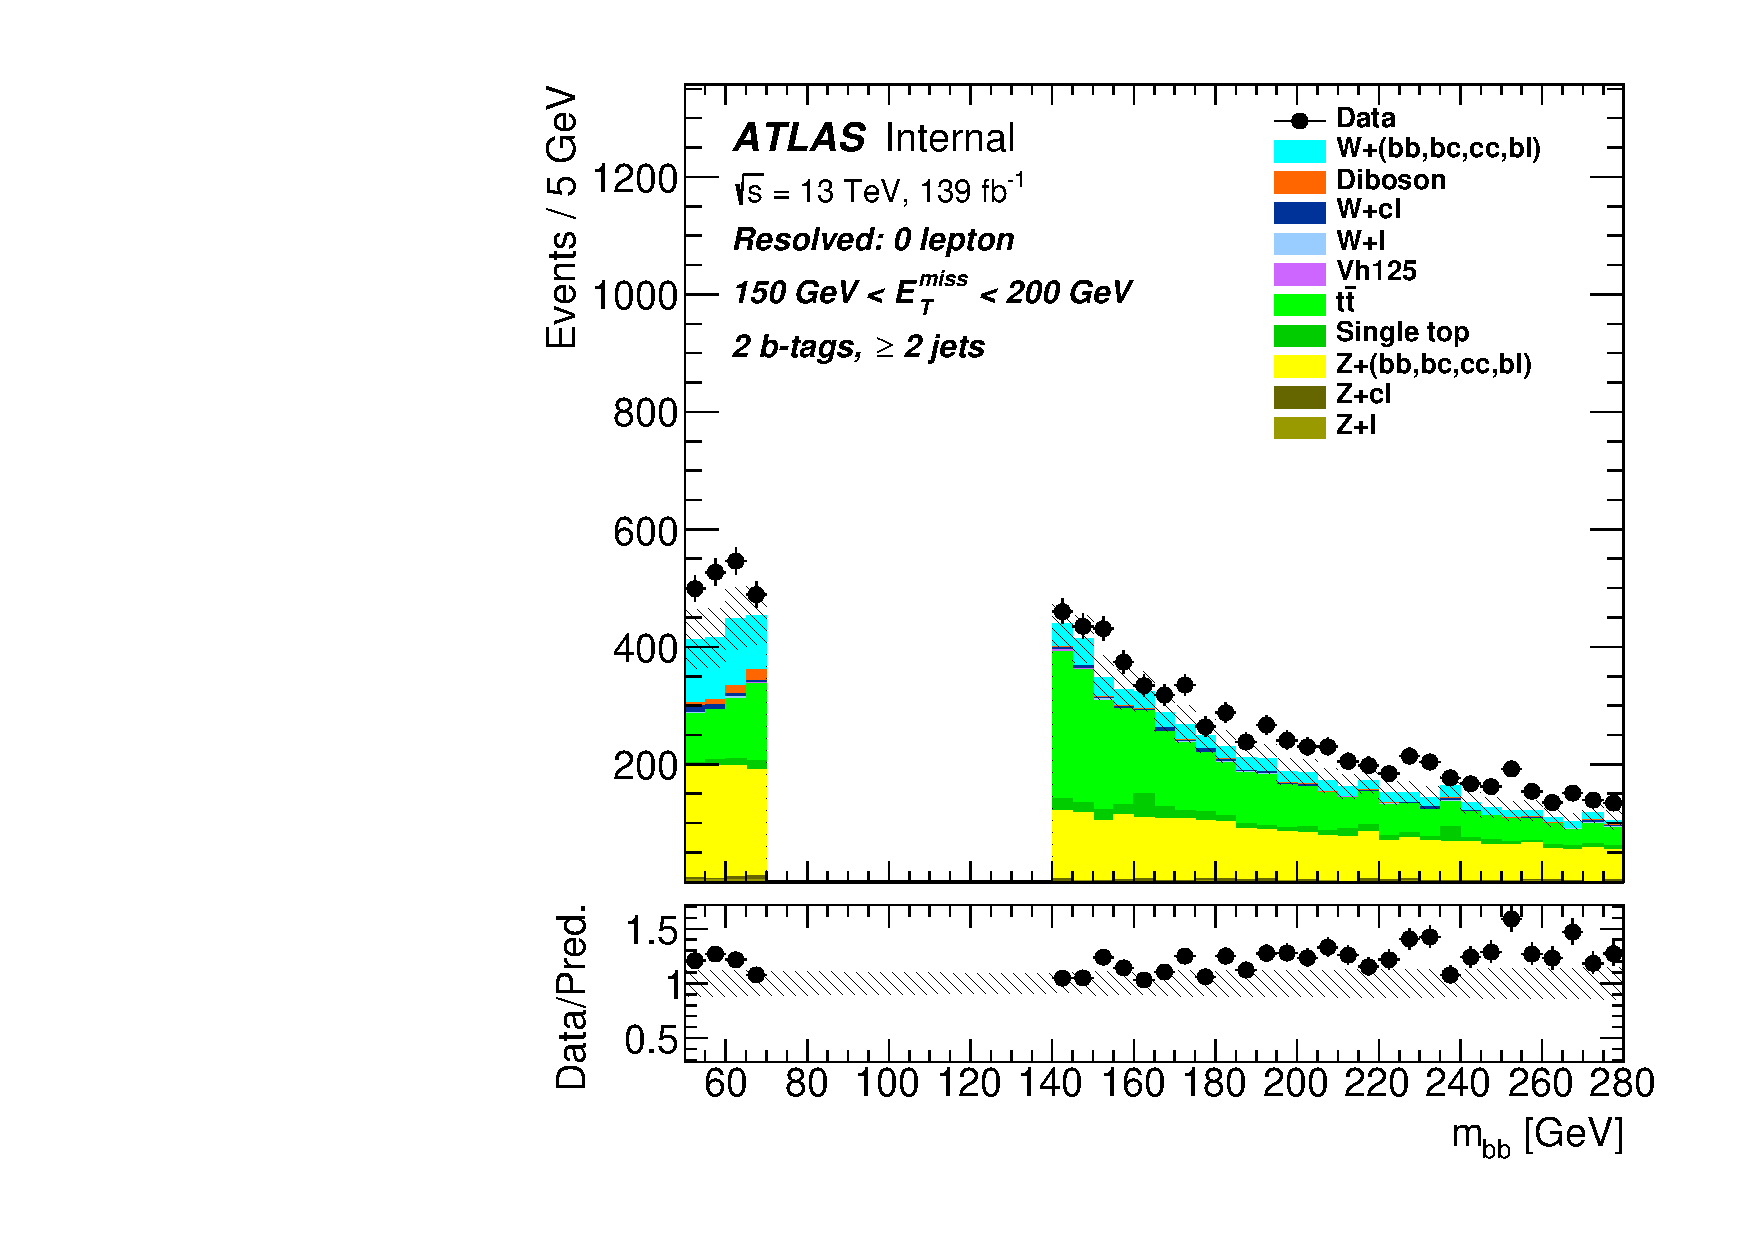
\includegraphics[width=0.46\linewidth]{chapters/c9/figures/Region_distmBB_J2_L0_T2_DSR_Y2015_incJet1_Fat0_incFat1_BMin150_BMax200_Prefit.pdf}
  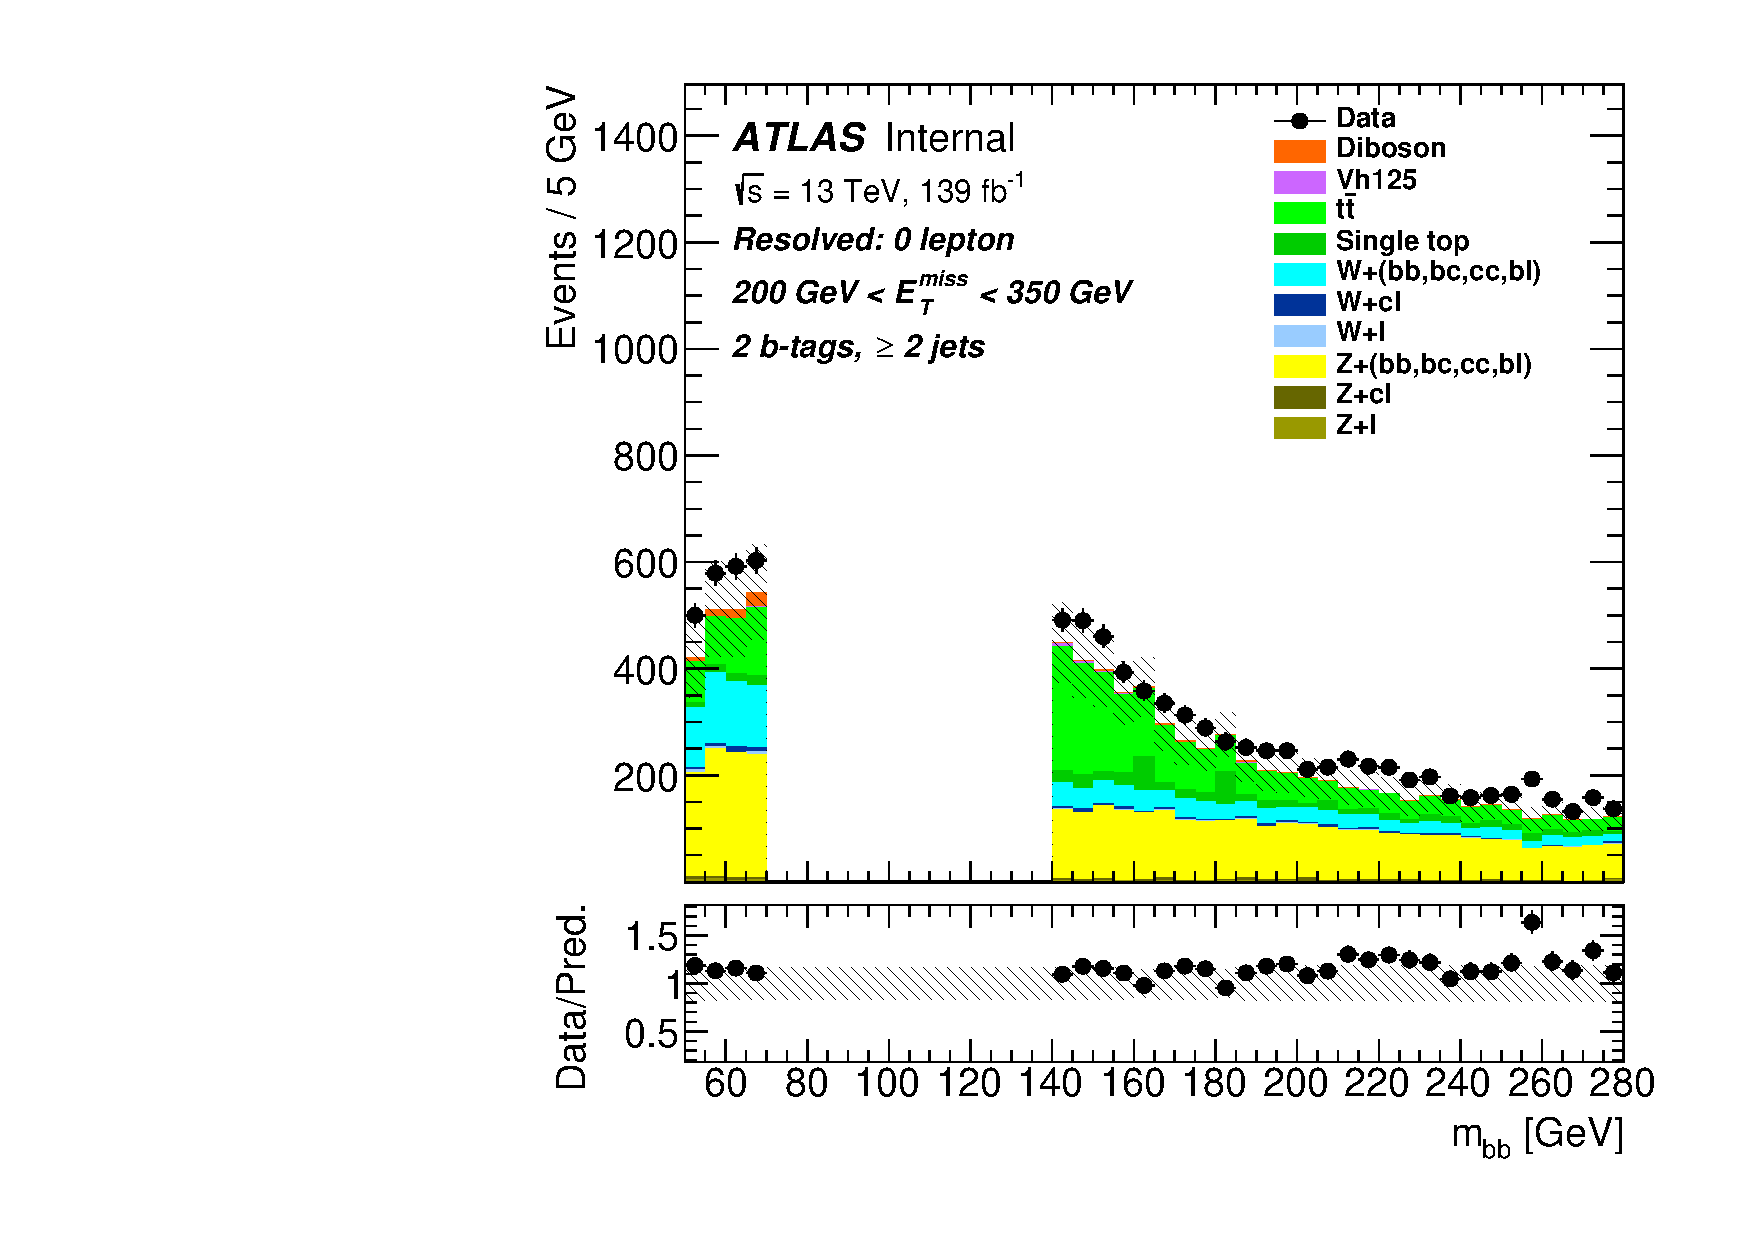
\includegraphics[width=0.46\linewidth]{chapters/c9/figures/Region_distmBB_J2_L0_T2_DSR_Y2015_incJet1_Fat0_incFat1_BMin200_BMax350_Prefit.pdf}\\
  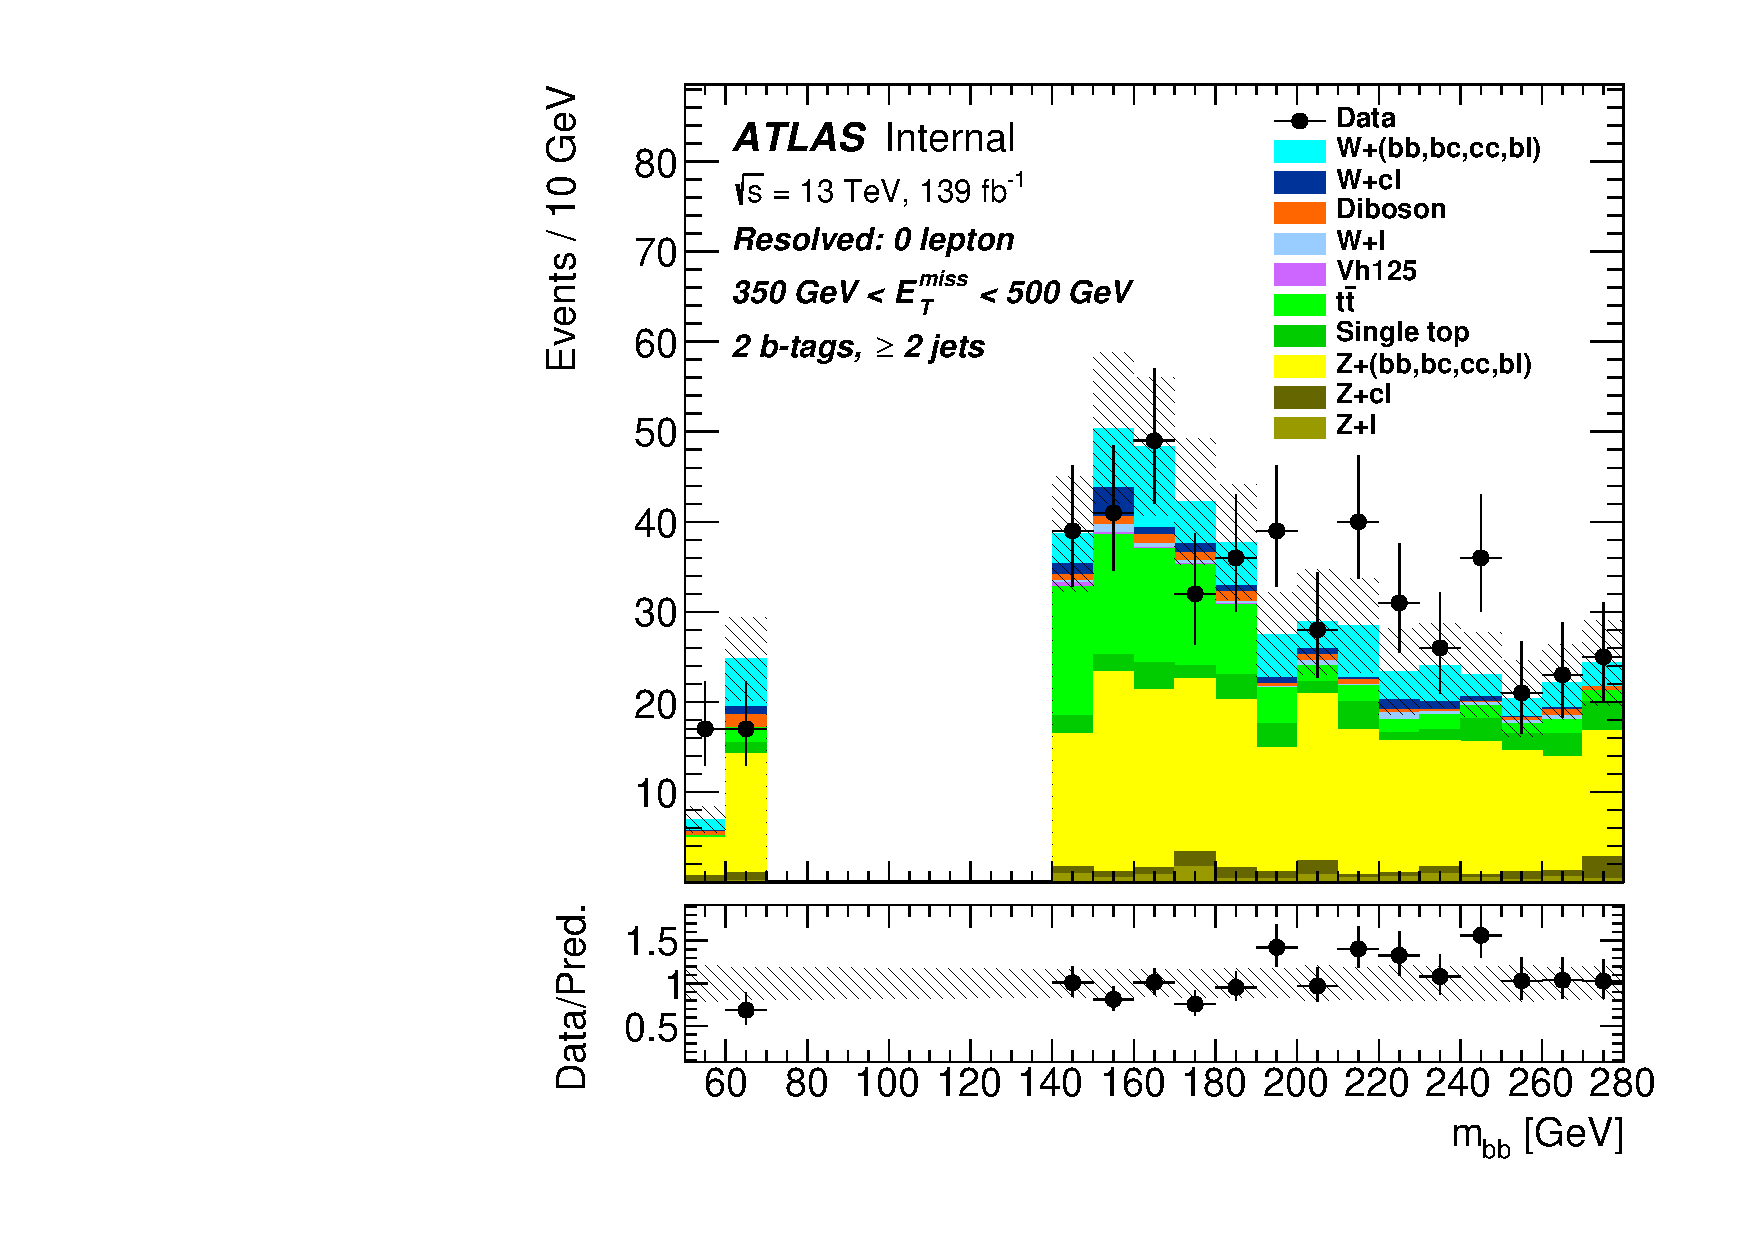
\includegraphics[width=0.46\linewidth]{chapters/c9/figures/Region_distmBB_J2_L0_T2_DSR_Y2015_incJet1_Fat0_incFat1_BMin350_BMax500_Prefit.pdf}
  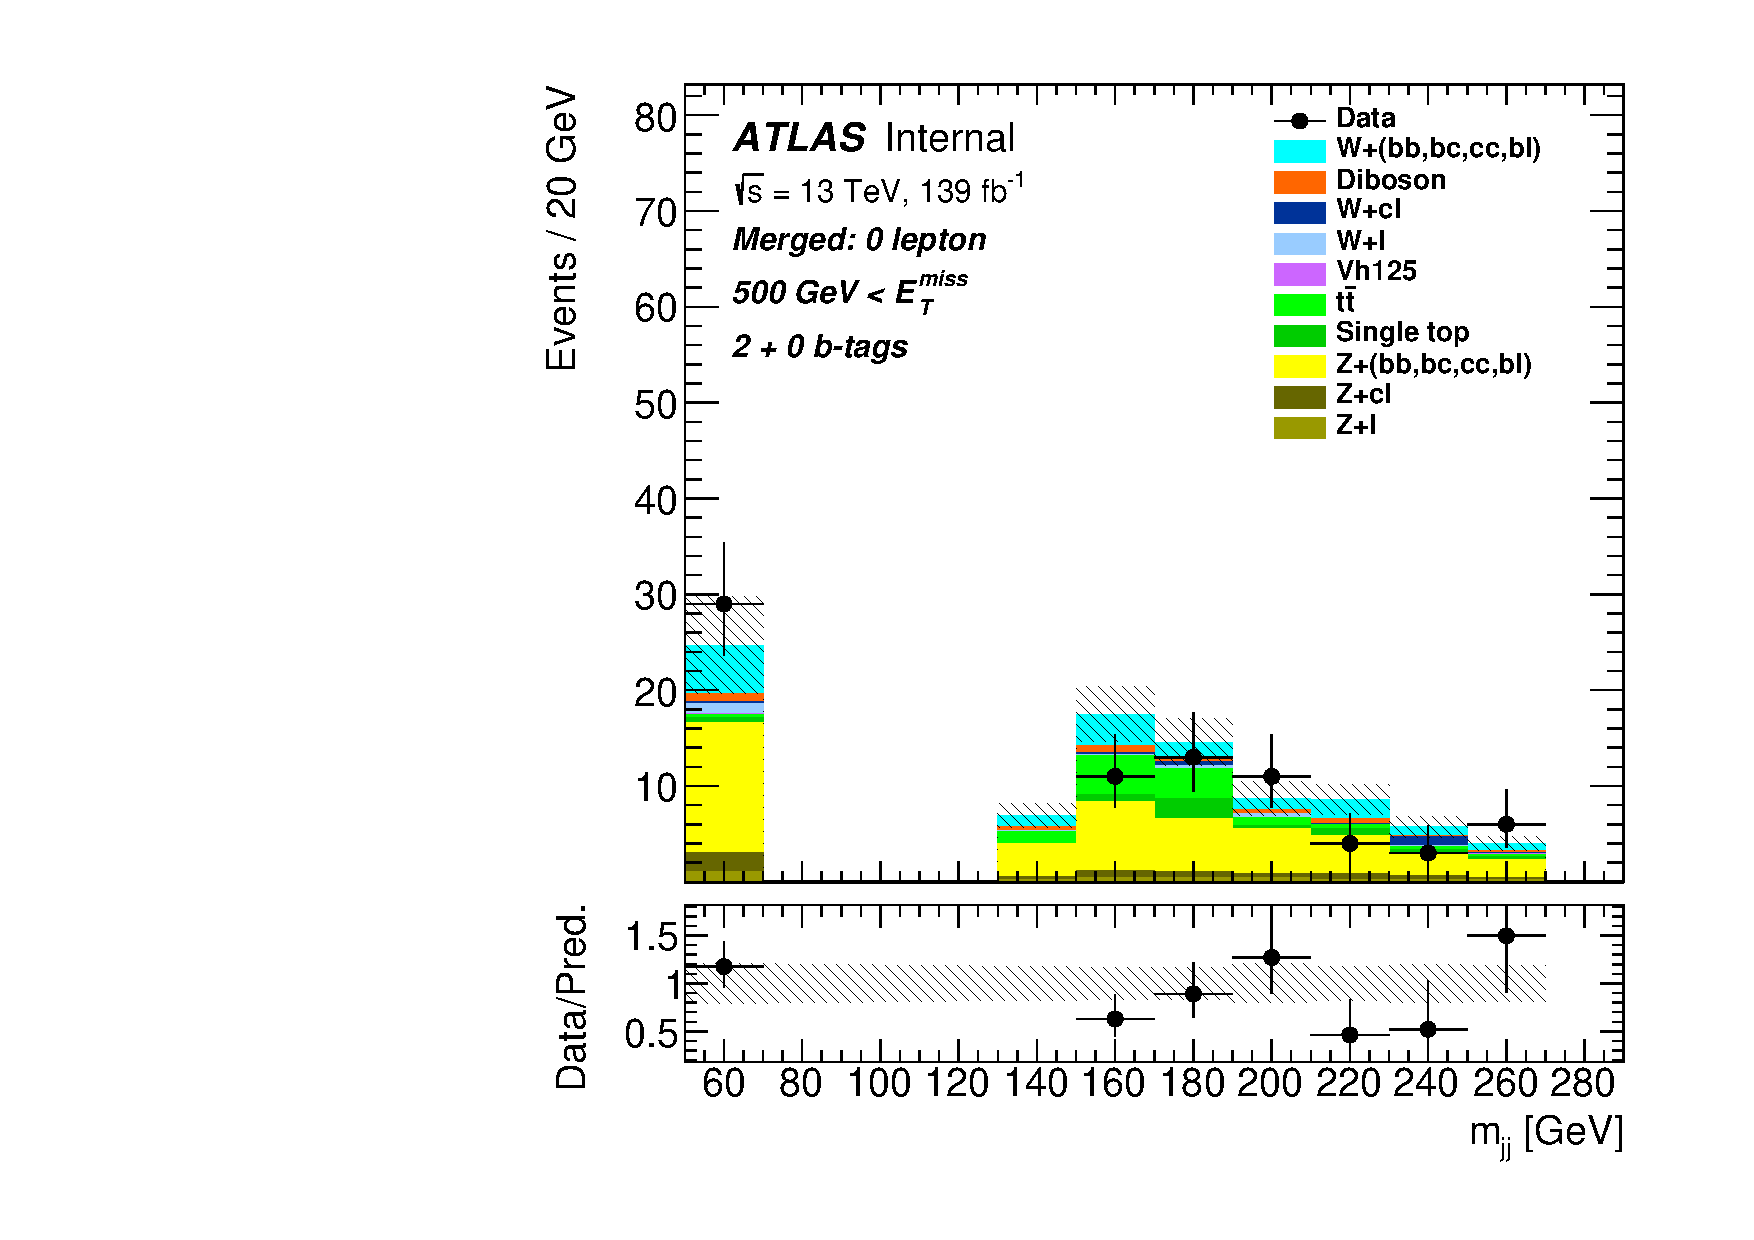
\includegraphics[width=0.46\linewidth]{chapters/c9/figures/Region_BMin500_incFat1_Fat1_incJet1_Y2015_DSR_T20_L0_distmBB_J0_Prefit.pdf}
\caption{Pre-fit Higgs candidate mass spectra in the different \met~regions with 2 b-tagged jets in the 0-lepton channel with 139~\ifb~data. The error band contains all the statistical and systematic uncertainties included in the fit.}
\label{fig:Data_MC_SR_m_jj_2b}
\end{figure}



\subsection{1-lepton (1L)}

\par In the 1-lepton control region, the muon charge distribution is used for the likelihood fit. As shown in Fig.~\ref{fig:Data_MC_CR1_mu_charge_2b}, the
dominant background contributions come from W + Heavy flavor jets and $t\bar{t}$. 
Since the $t\bar{t}$ process is charge-symmetric, while the W + jets process is expected to produce a surplus of positive muons, 
fitting the muon charge is expected to constrain the W + Heavy flavor normalisation.

\begin{figure}[H]
  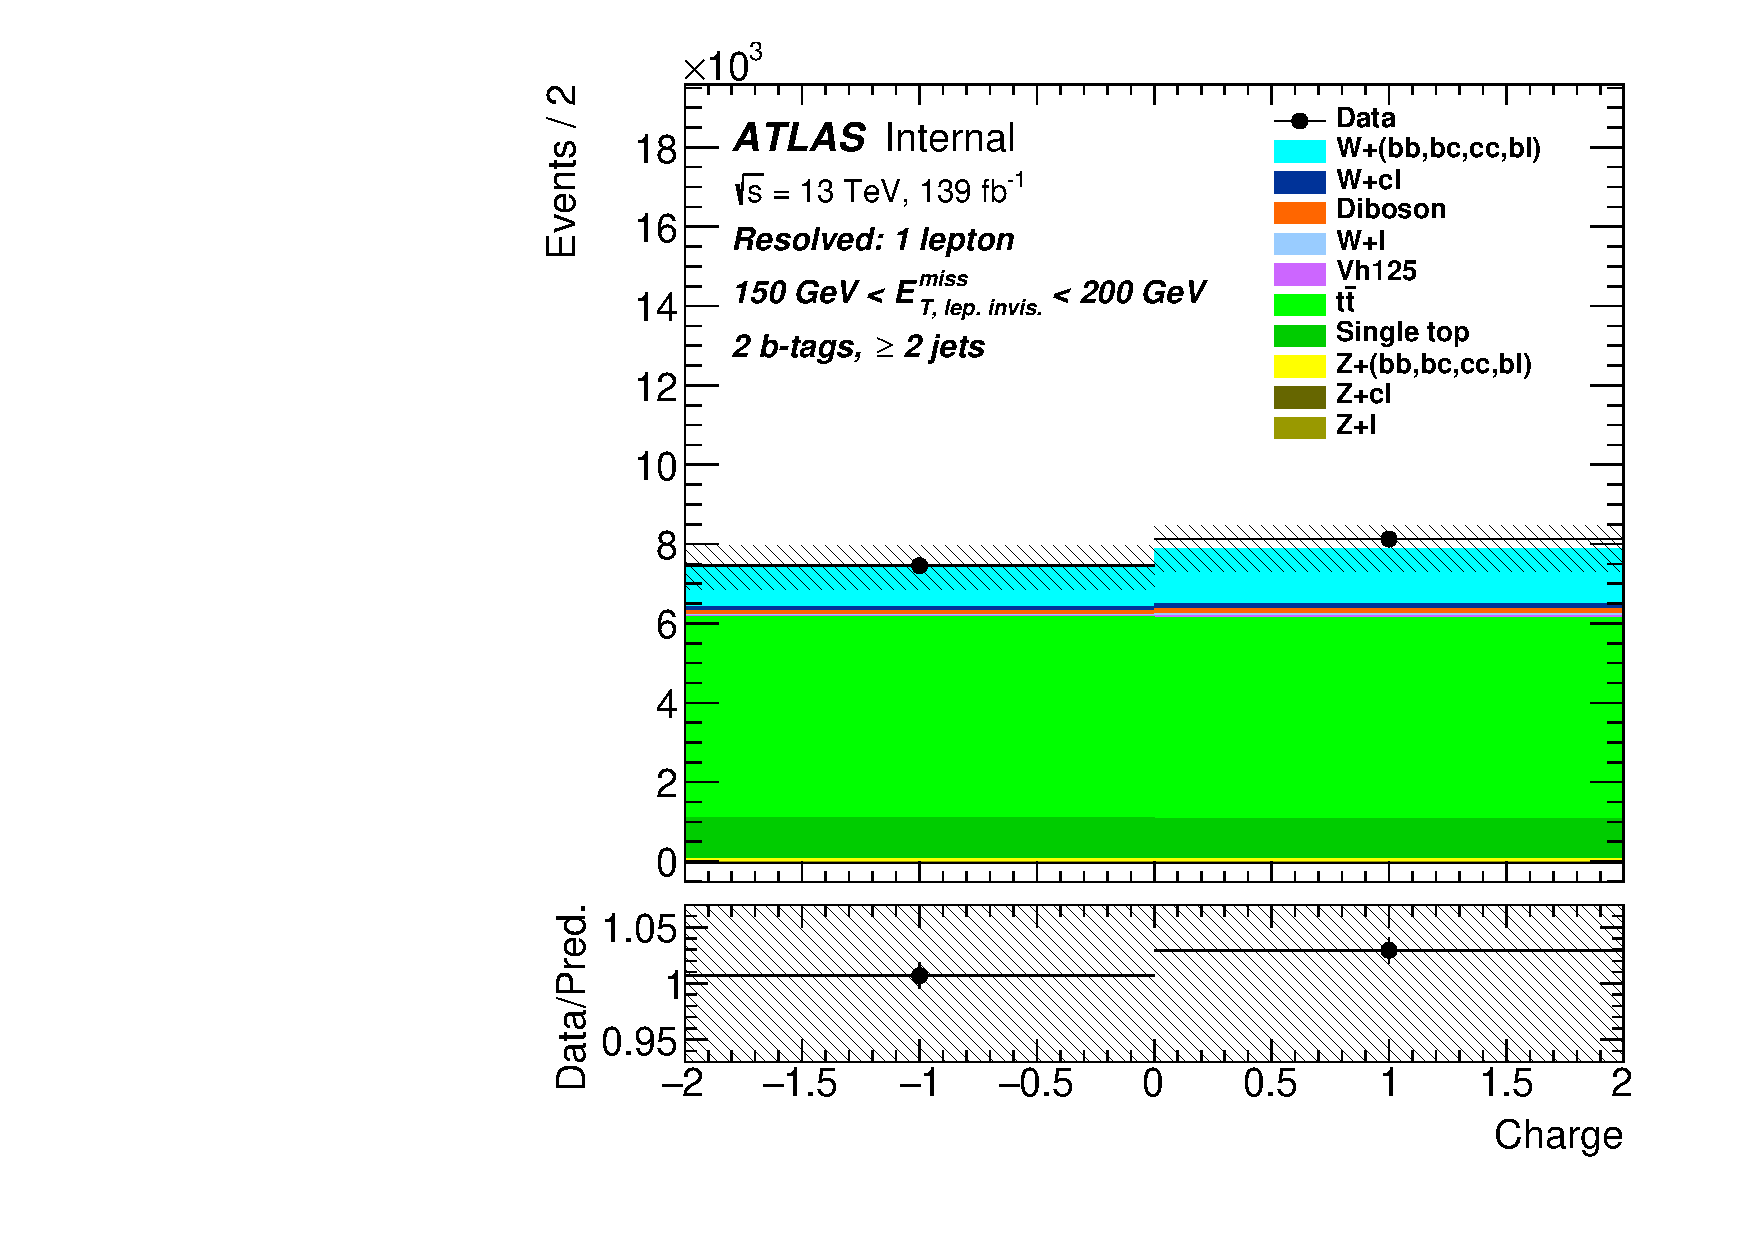
\includegraphics[width=0.46\linewidth]{chapters/c9/figures/Region_distCharge_J2_L1_T2_DCR1_Y2015_incJet1_Fat0_incFat1_BMin150_BMax200_Prefit.pdf}
  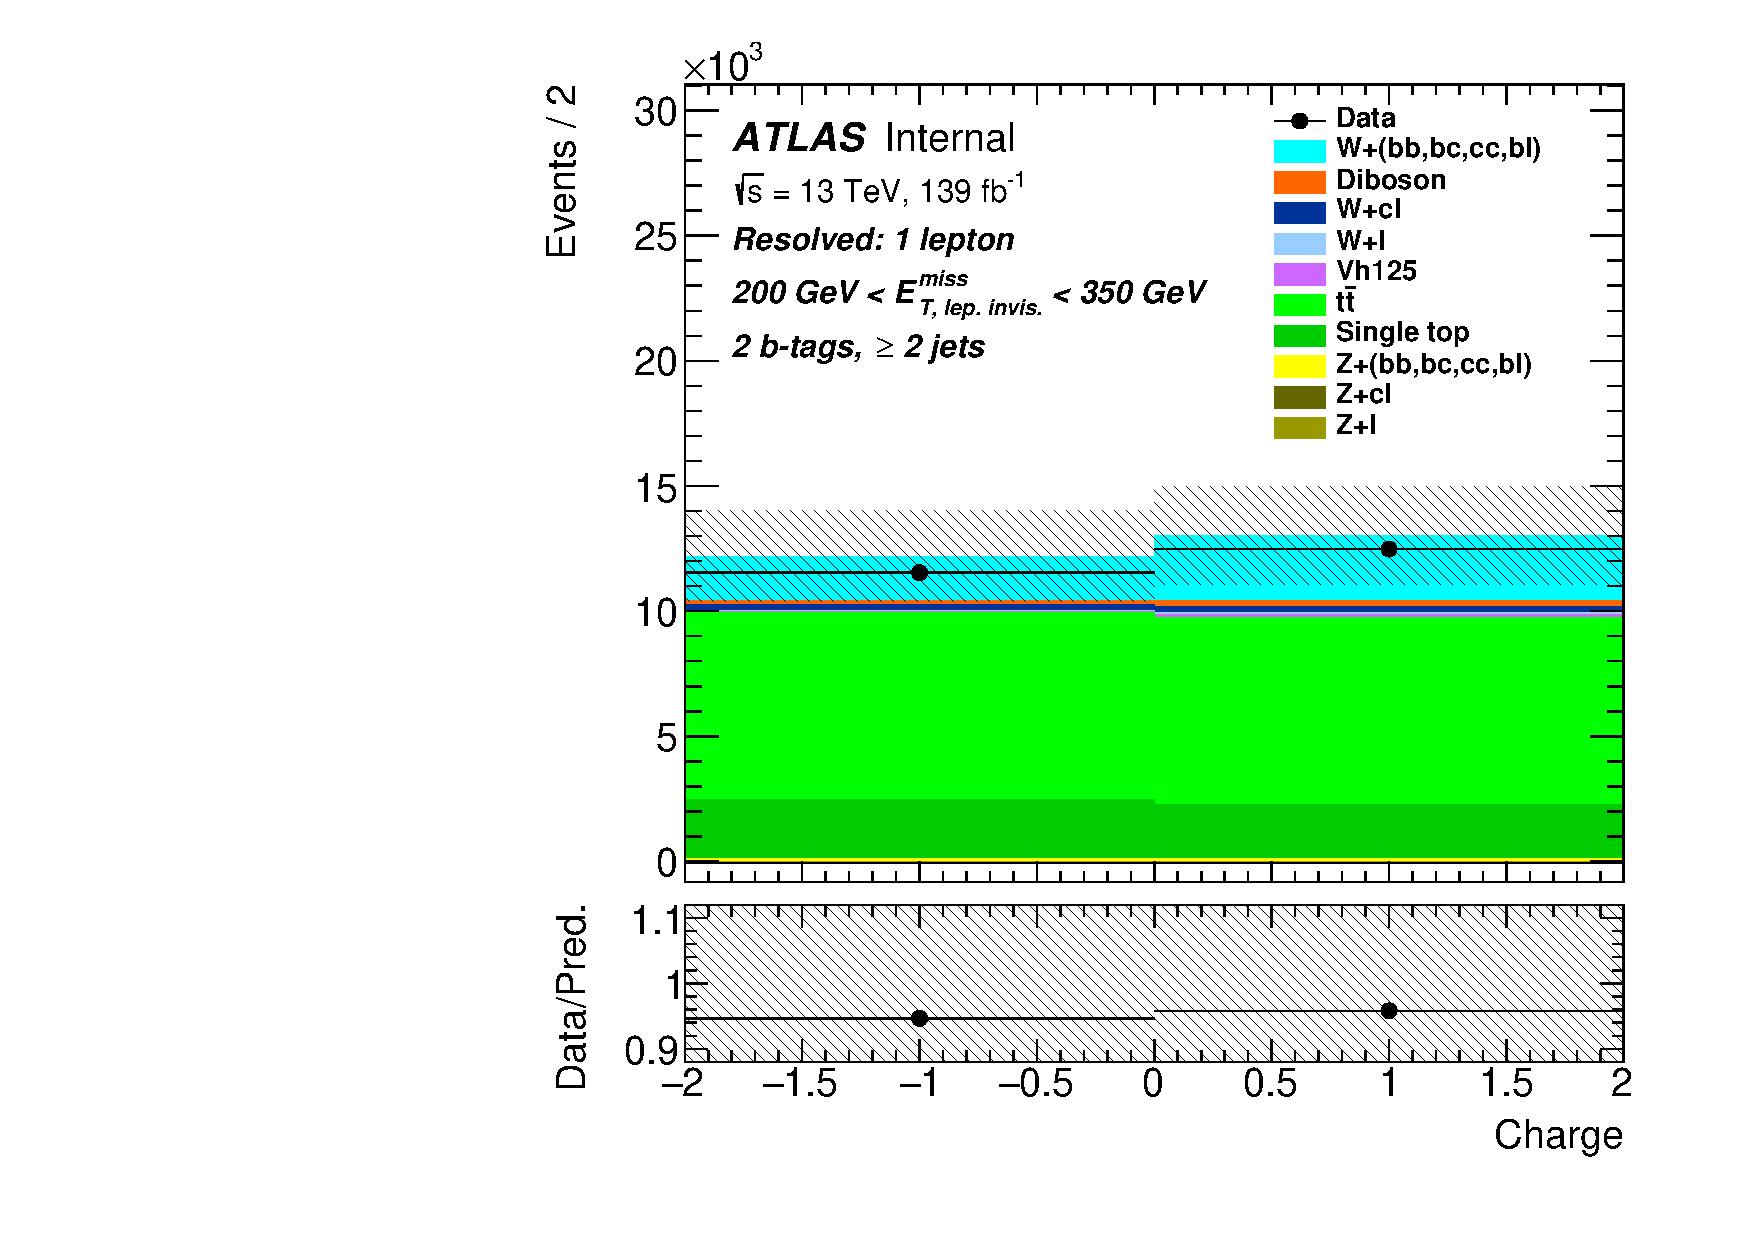
\includegraphics[width=0.46\linewidth]{chapters/c9/figures/Region_distCharge_J2_L1_T2_DCR1_Y2015_incJet1_Fat0_incFat1_BMin200_BMax350_Prefit.pdf}\\
  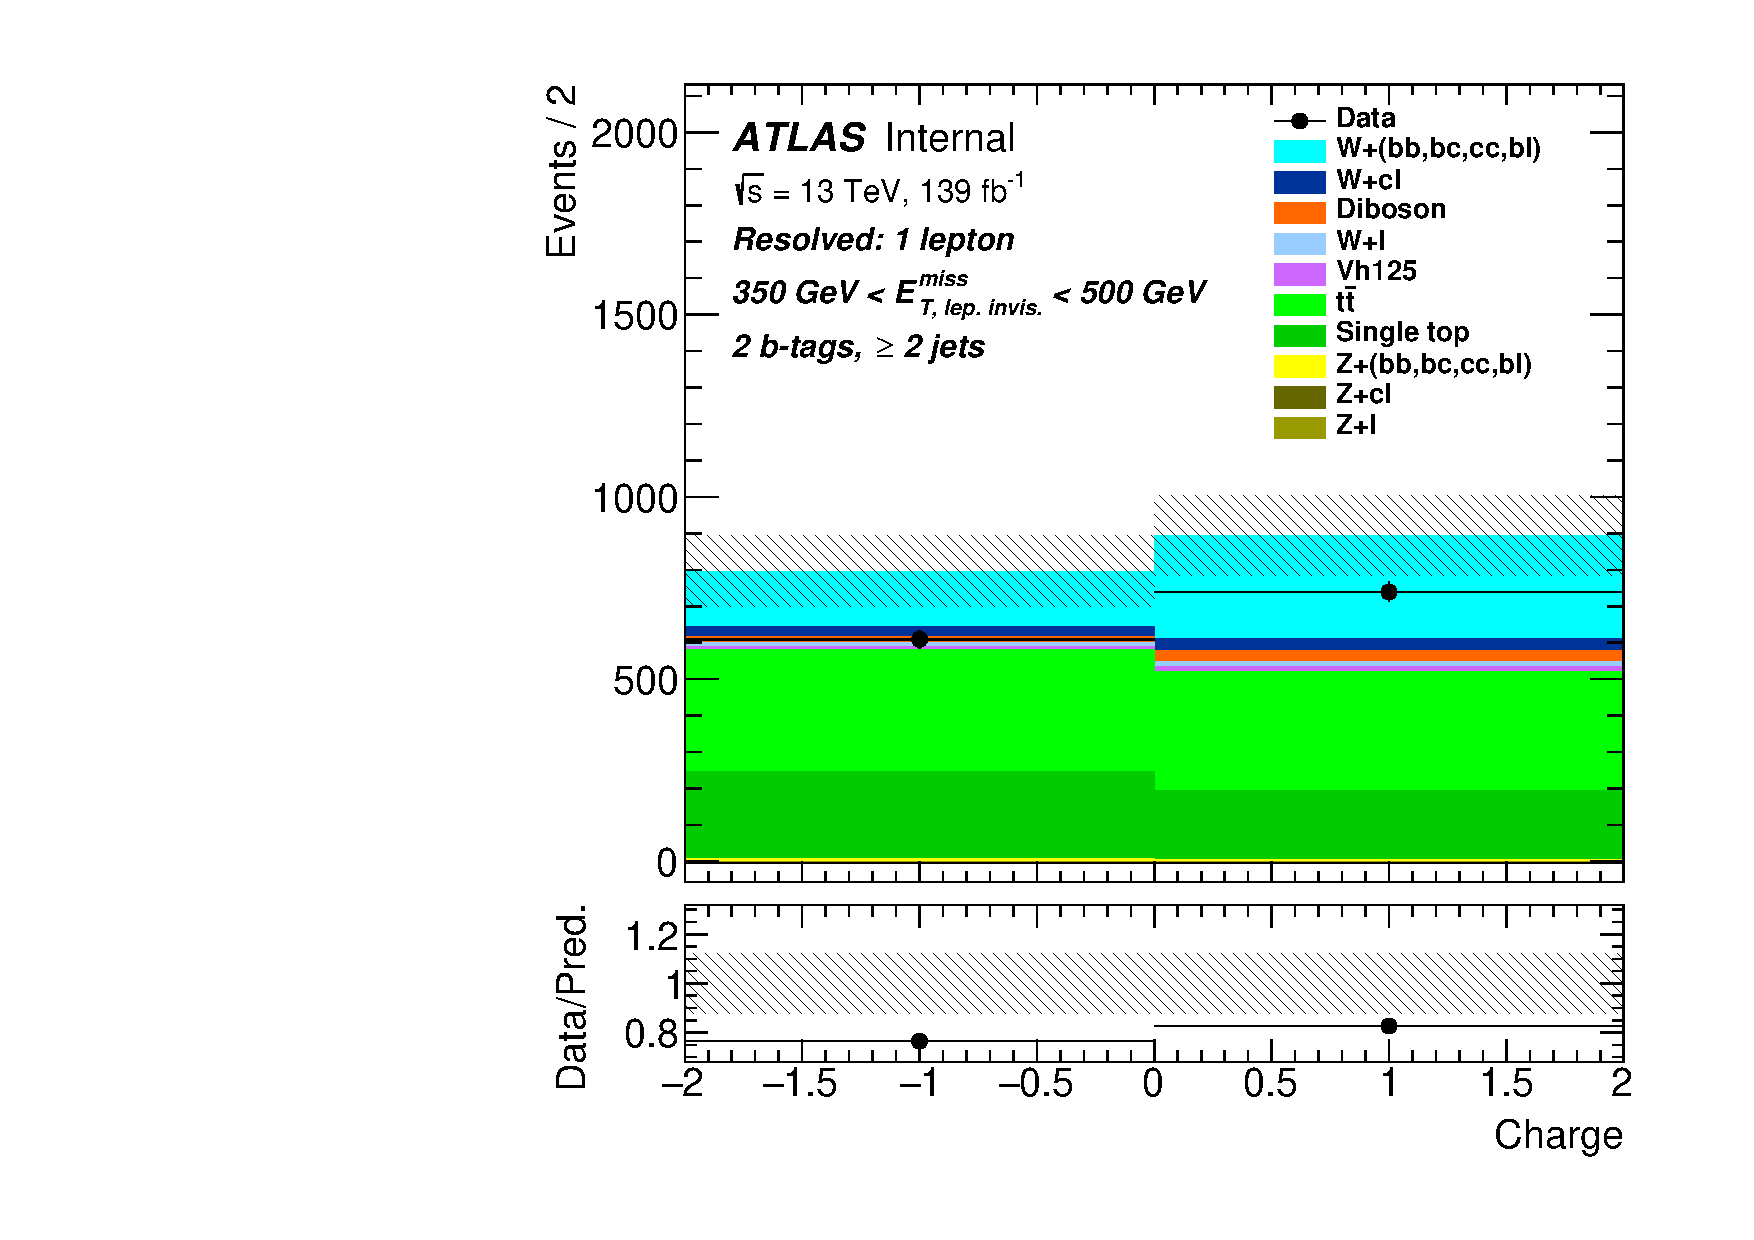
\includegraphics[width=0.46\linewidth]{chapters/c9/figures/Region_distCharge_J2_L1_T2_DCR1_Y2015_incJet1_Fat0_incFat1_BMin350_BMax500_Prefit.pdf}
  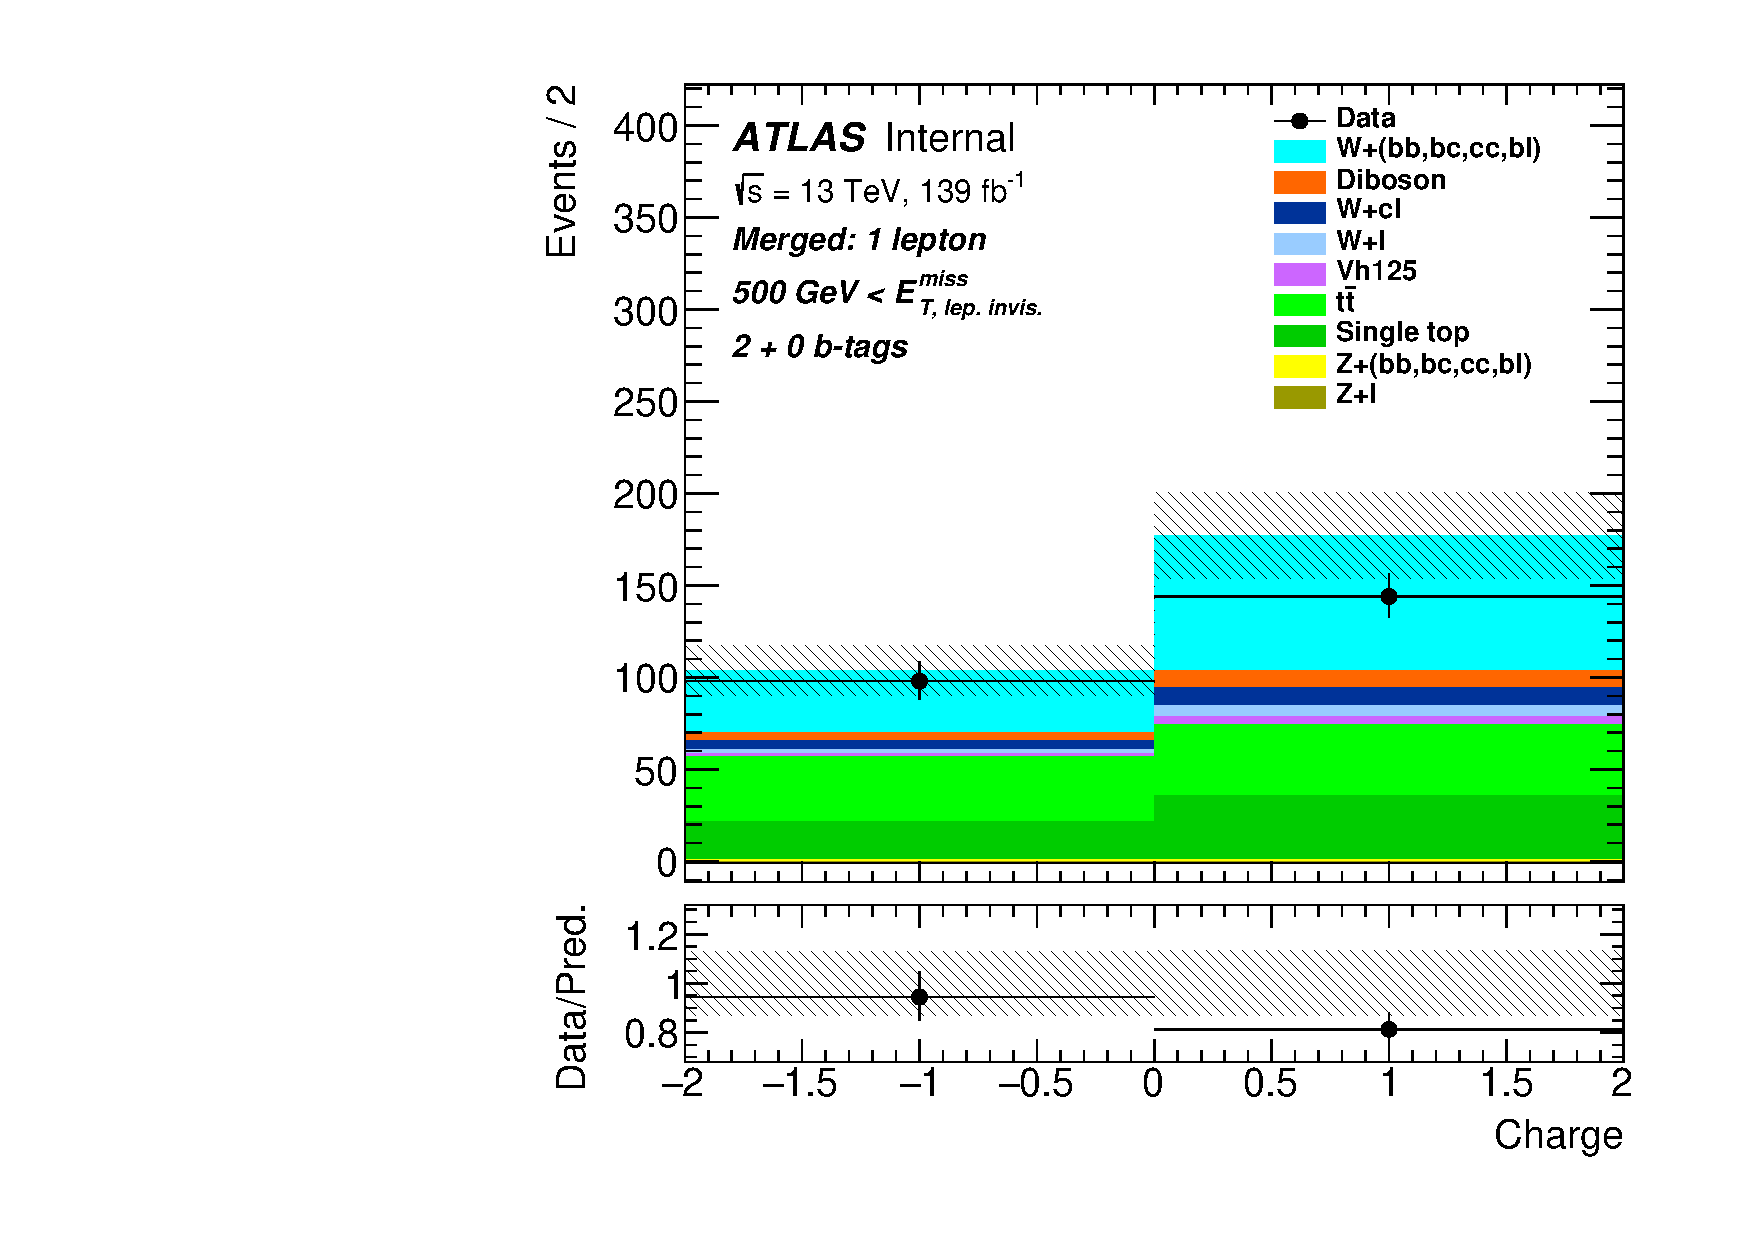
\includegraphics[width=0.46\linewidth]{chapters/c9/figures/Region_BMin500_incFat1_Fat1_incJet1_Y2015_DCR1_T20_L1_distCharge_J0_Prefit.pdf}
\caption{Pre-fit distribution of the muon charge in the different \met~regions with \\2 b-tagged jets in the 1-lepton channel with 139~\ifb~data. The error band contains all the statistical and 
    systematic uncertainties included in the fit.}
\label{fig:Data_MC_CR1_mu_charge_2b}
\end{figure}
\subsection{2-lepton (2L)}
\par In the 2-lepton control region (combining ee and $\mu\mu$ channels), a fit of invariant mass are used as fitting input as shown in Fig.~\ref{fig:Data_MC_CR2_ll_m_jj_2b}. 
\par Since the region is dominated by Z + Heavy flavor jets, the underestimation of the Z + Heavy flavor production rate in MC is obvious. The overall underestimation of 
the Z + Heavy flavor rate will be corrected by the floating Z + Heavy flavor normalisation in the final fit. The ratio of data/MC yield is \met-dependent, and this will not be fixed with a single normalisation factor, a pull of the \met~uncertainties applied on the
Z + Heavy flavor sample is expected in the fit.
\begin{figure}[H]
  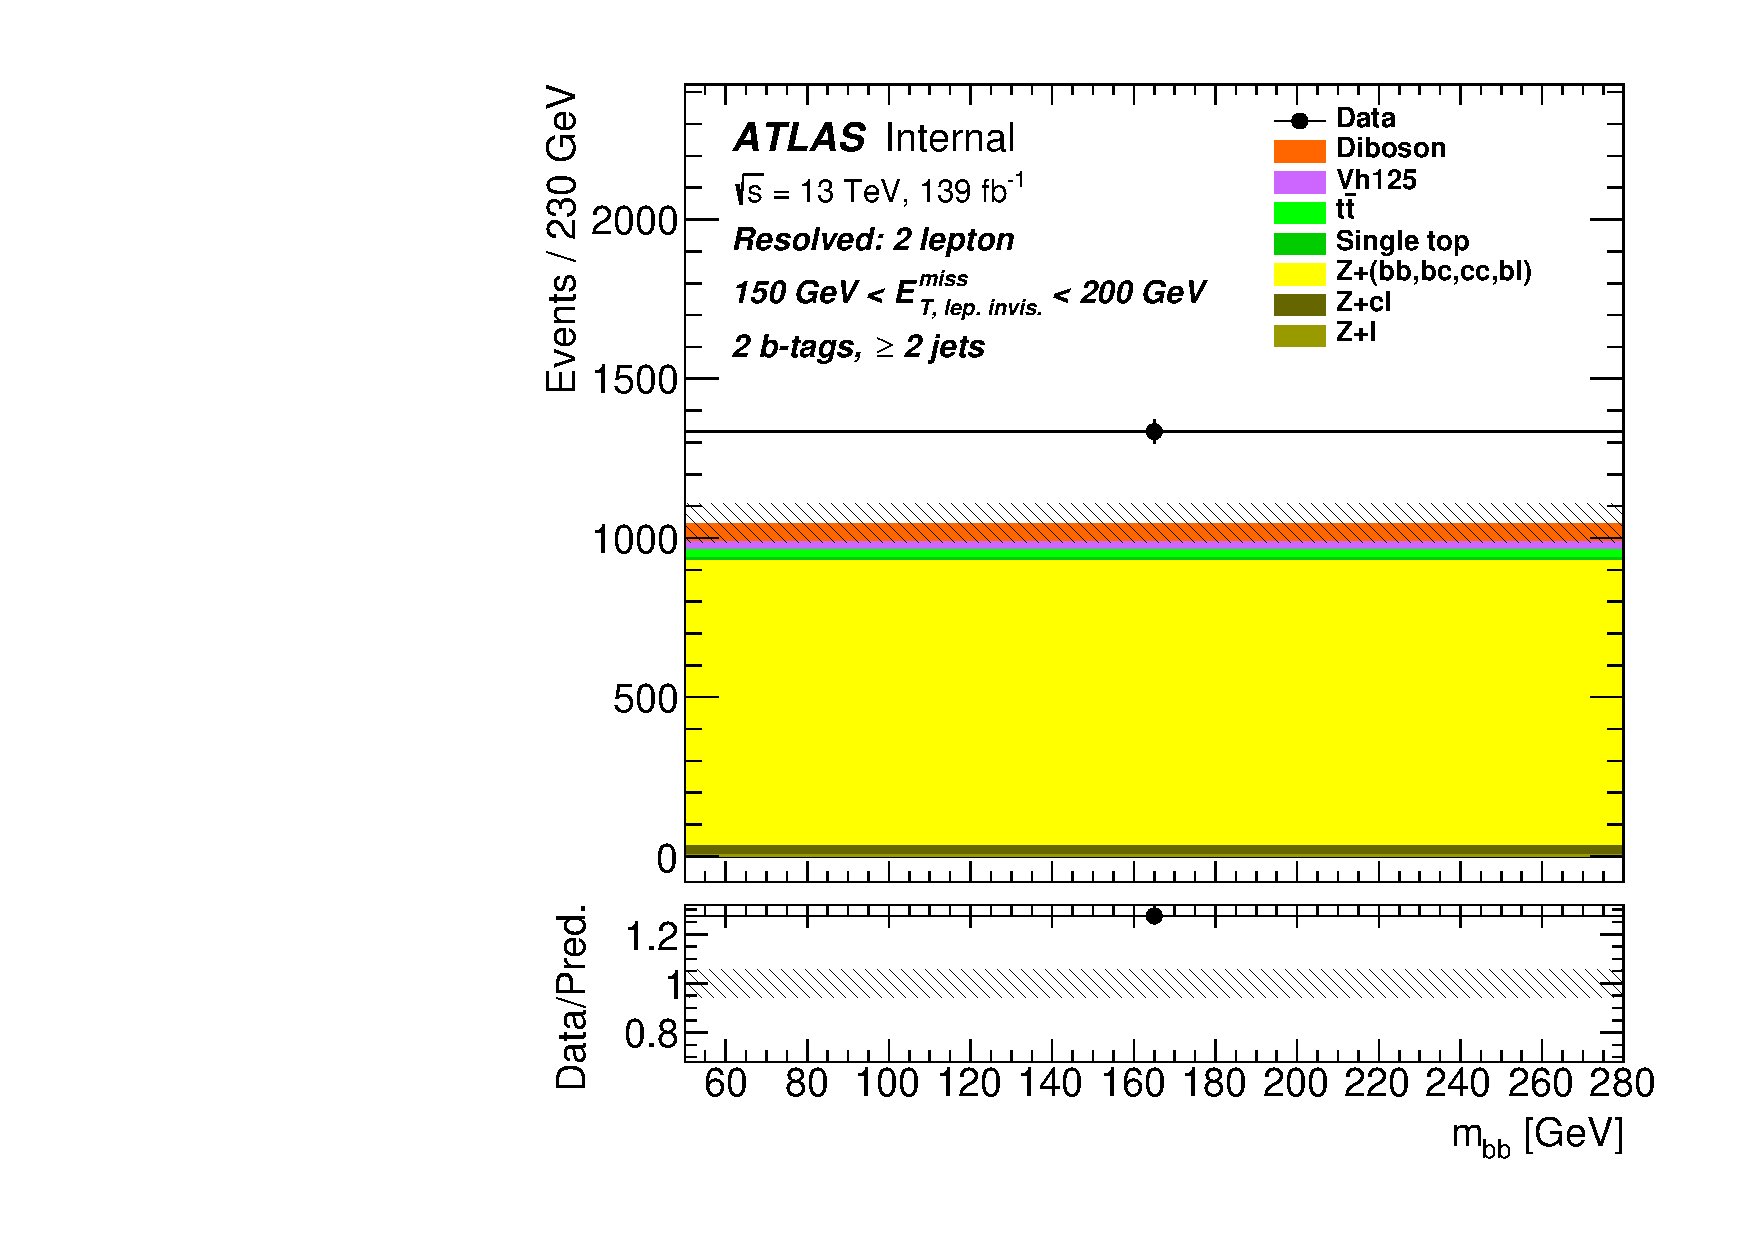
\includegraphics[width=0.46\linewidth]{chapters/c9/figures/Region_distmBB_J2_L2_T2_DCR2_Y2015_incJet1_Fat0_incFat1_BMin150_BMax200_Prefit.pdf}
  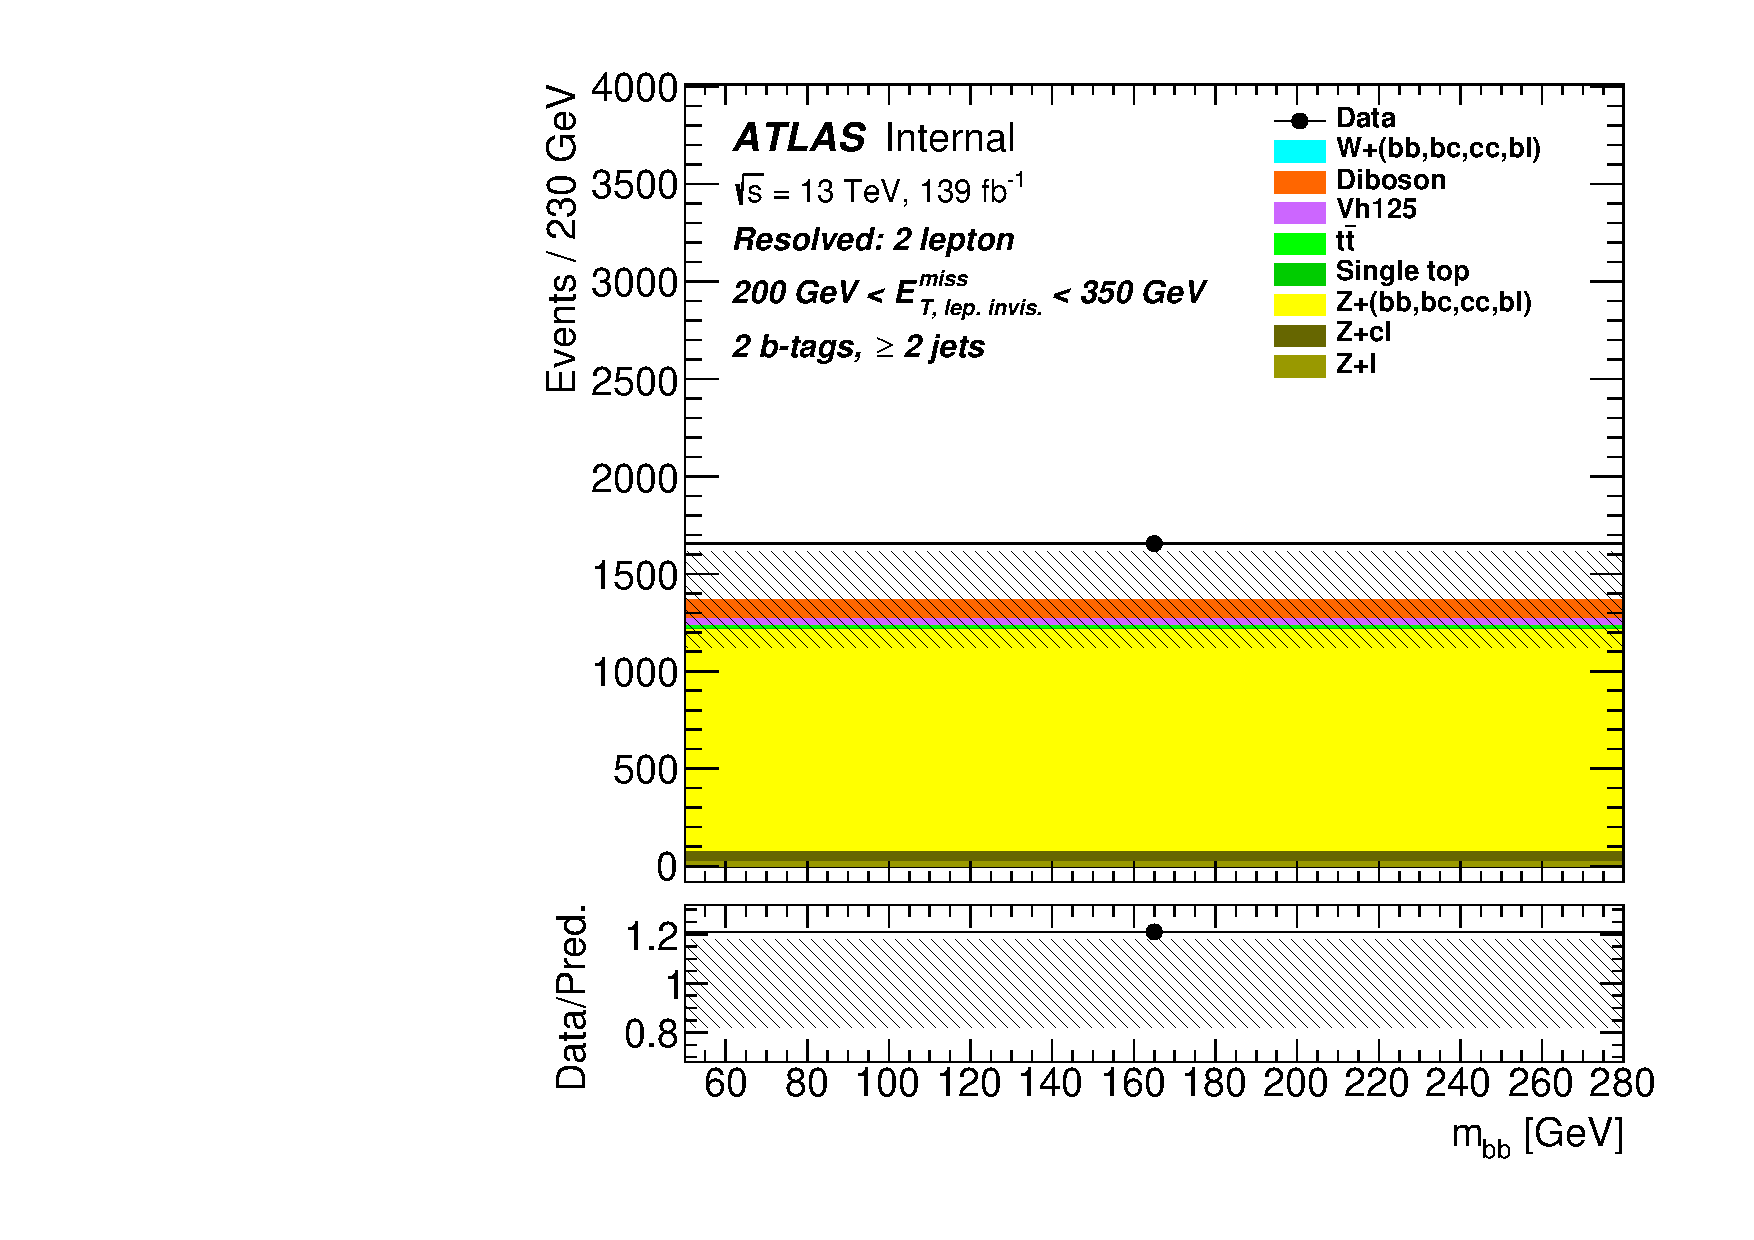
\includegraphics[width=0.46\linewidth]{chapters/c9/figures/Region_distmBB_J2_L2_T2_DCR2_Y2015_incJet1_Fat0_incFat1_BMin200_BMax350_Prefit.pdf}\\
  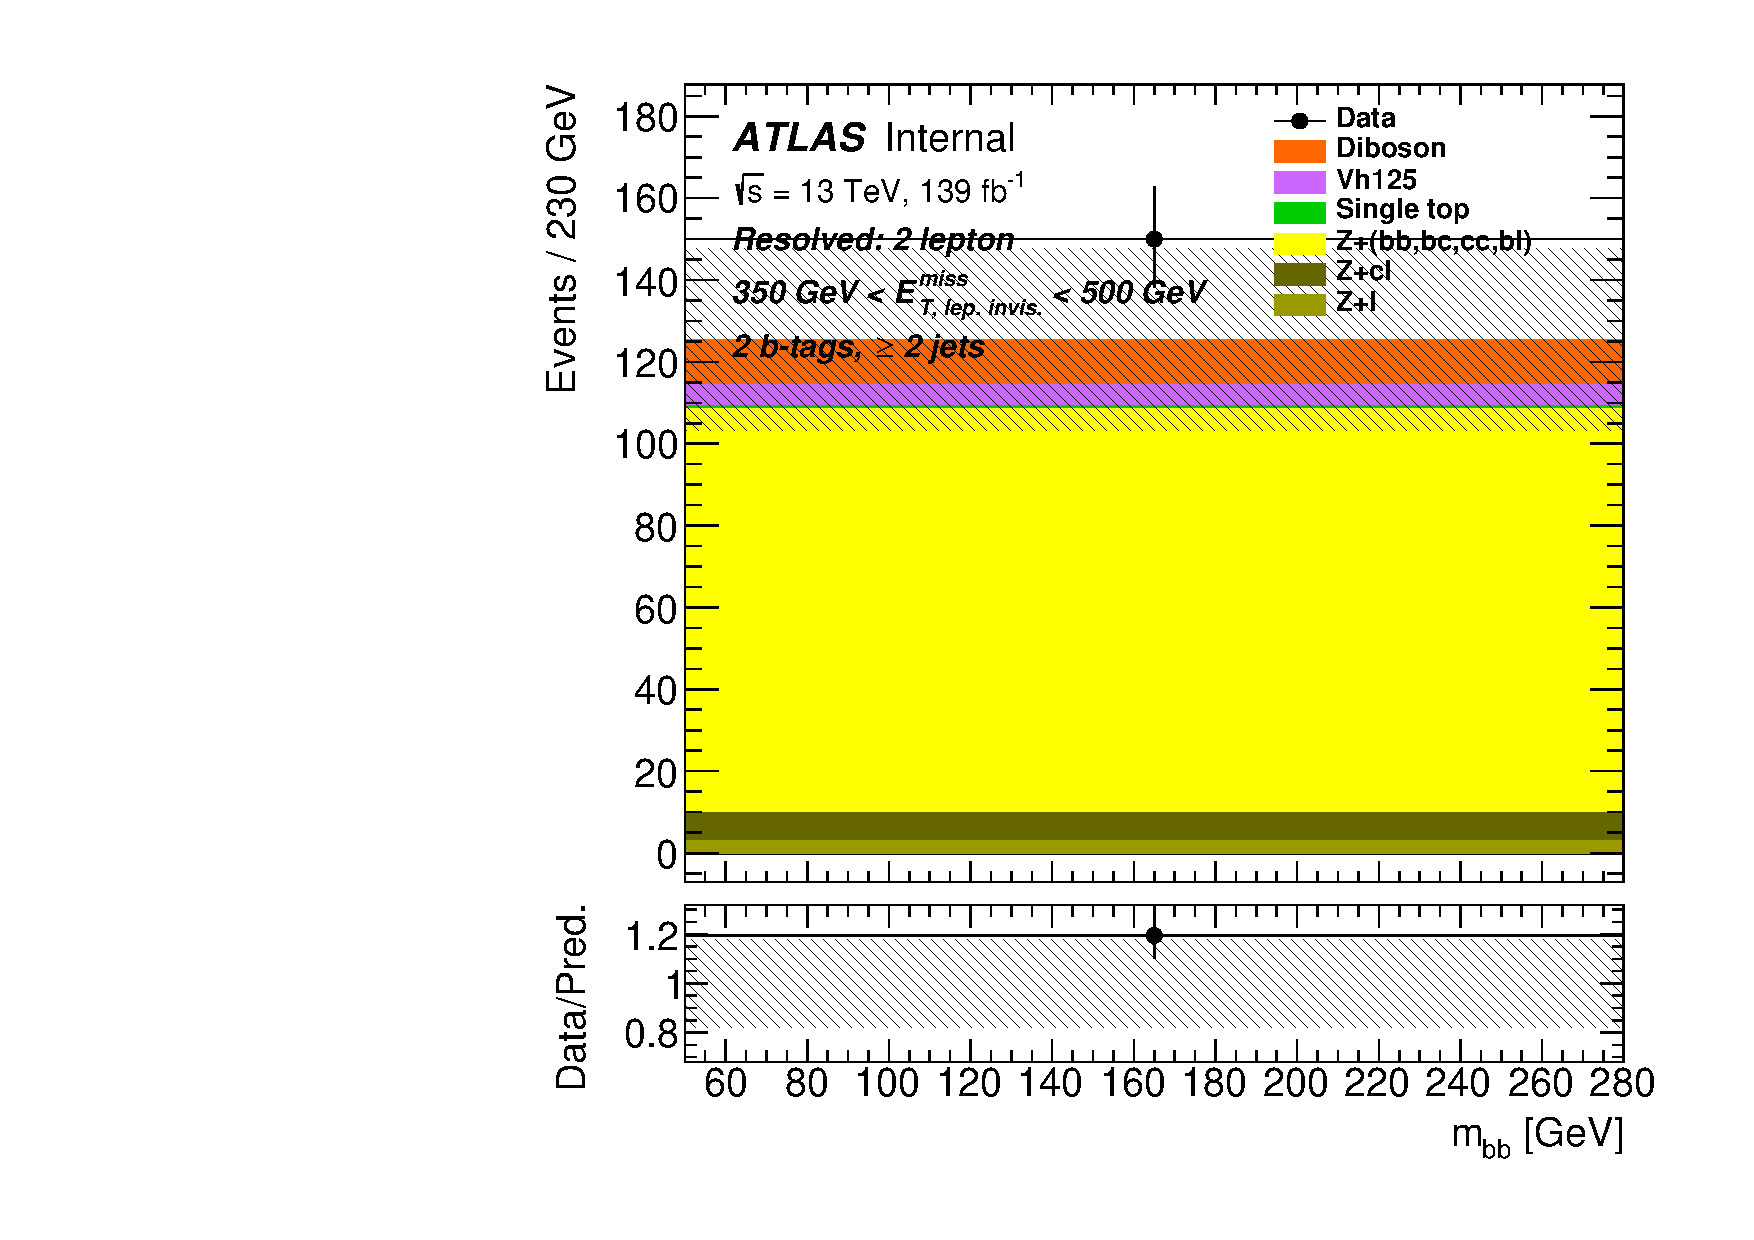
\includegraphics[width=0.46\linewidth]{chapters/c9/figures/Region_distmBB_J2_L2_T2_DCR2_Y2015_incJet1_Fat0_incFat1_BMin350_BMax500_Prefit.pdf}
  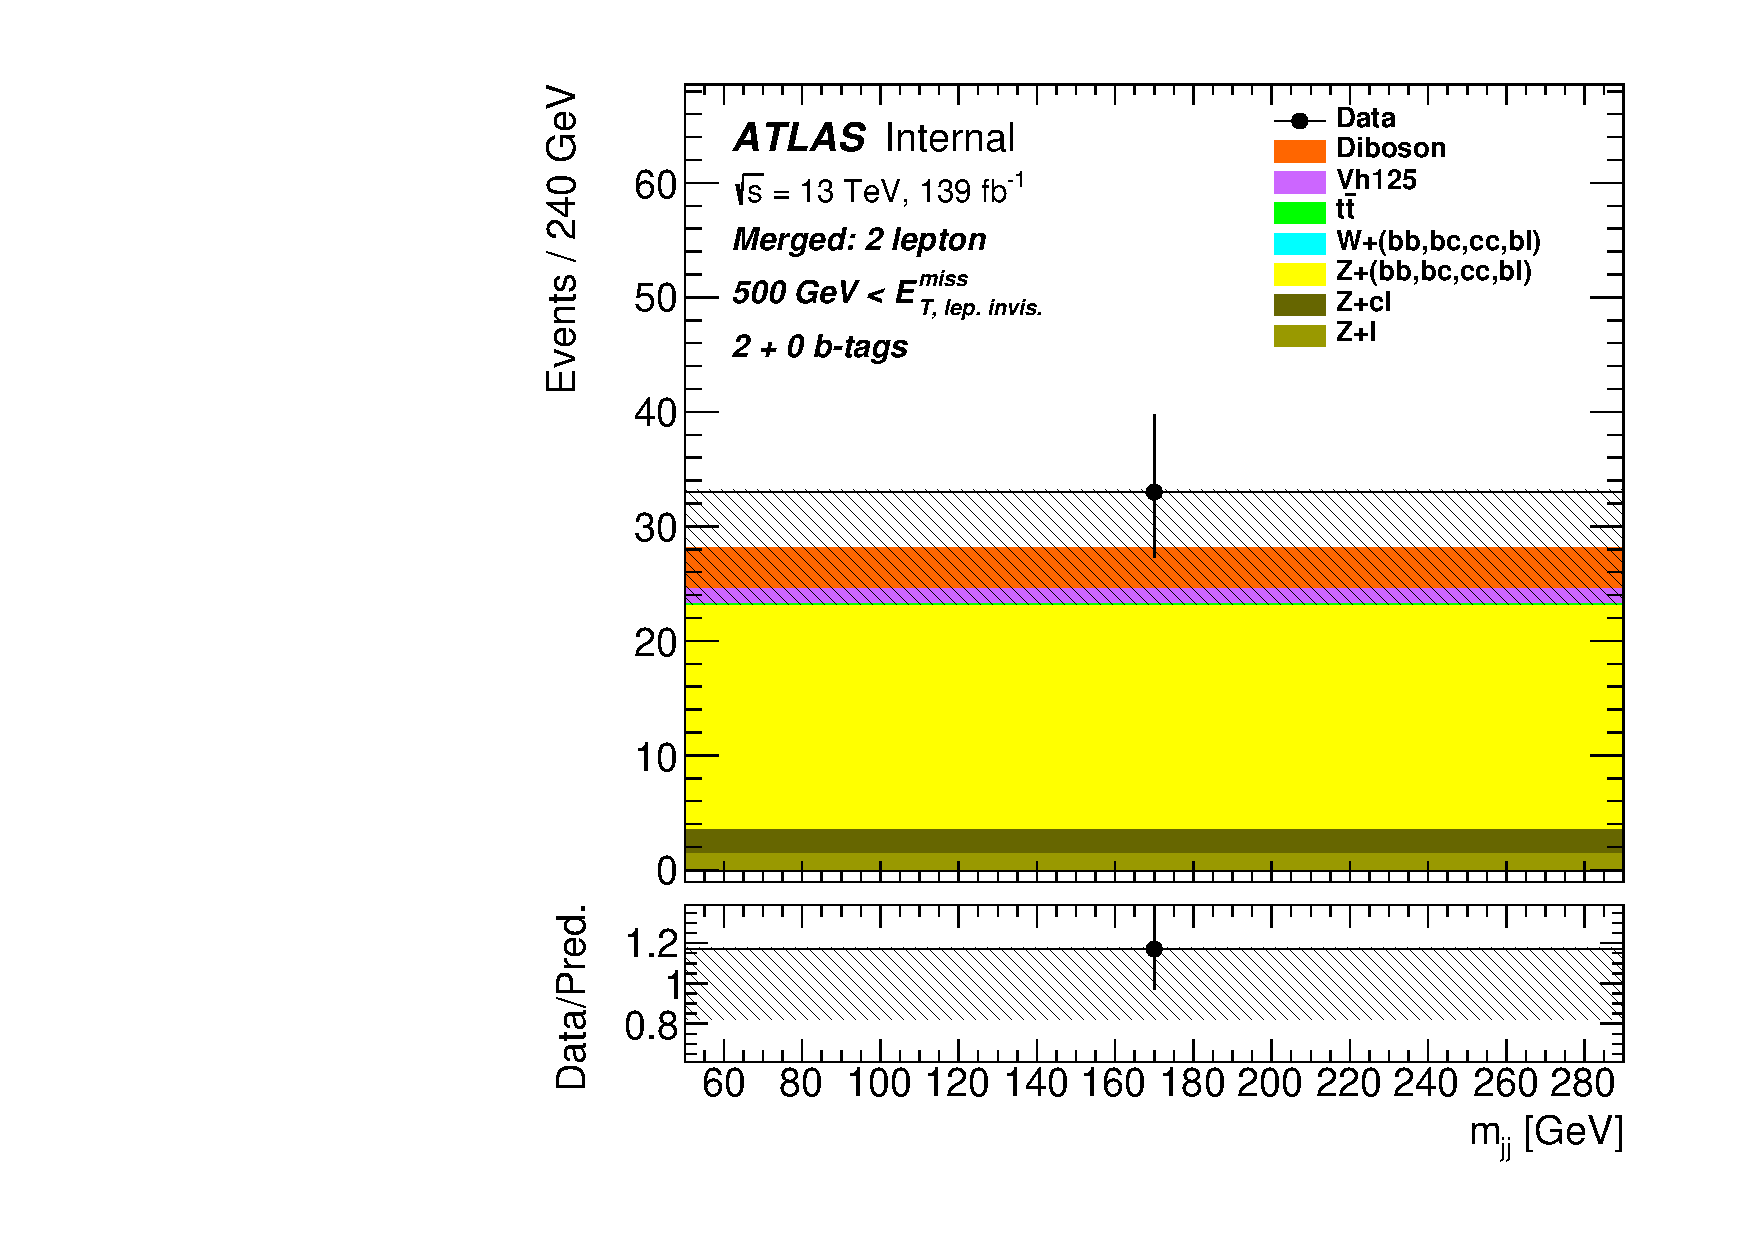
\includegraphics[width=0.46\linewidth]{chapters/c9/figures/Region_BMin500_incFat1_Fat1_incJet1_Y2015_DCR2_T20_L2_distmBB_J0_Prefit.pdf}
\caption{Total yields in the 2-lepton control region for different \met~regions with \\2 b-tagged jets before the combined signal and control region background-only fit with 139~\ifb~data.}
\label{fig:Data_MC_CR2_ll_m_jj_2b}
\end{figure}

\section{Post-fit results}
\par For 79.8~\ifb, the post-fit unblinded distributions of fitting inputs in the 0, 1 and 2-lepton channels are shown in Fig.~\ref{fig:Data_MC_SR_m_jj_2b_postfit}, Fig.~\ref{fig:Data_MC_CR1_mu_charge_2b_postfit} and Fig.~\ref{fig:Data_MC_CR2_ll_m_jj_2b_postfit}.
\subsection{0-lepton (0L)}
\begin{figure}[H]
  \centering
    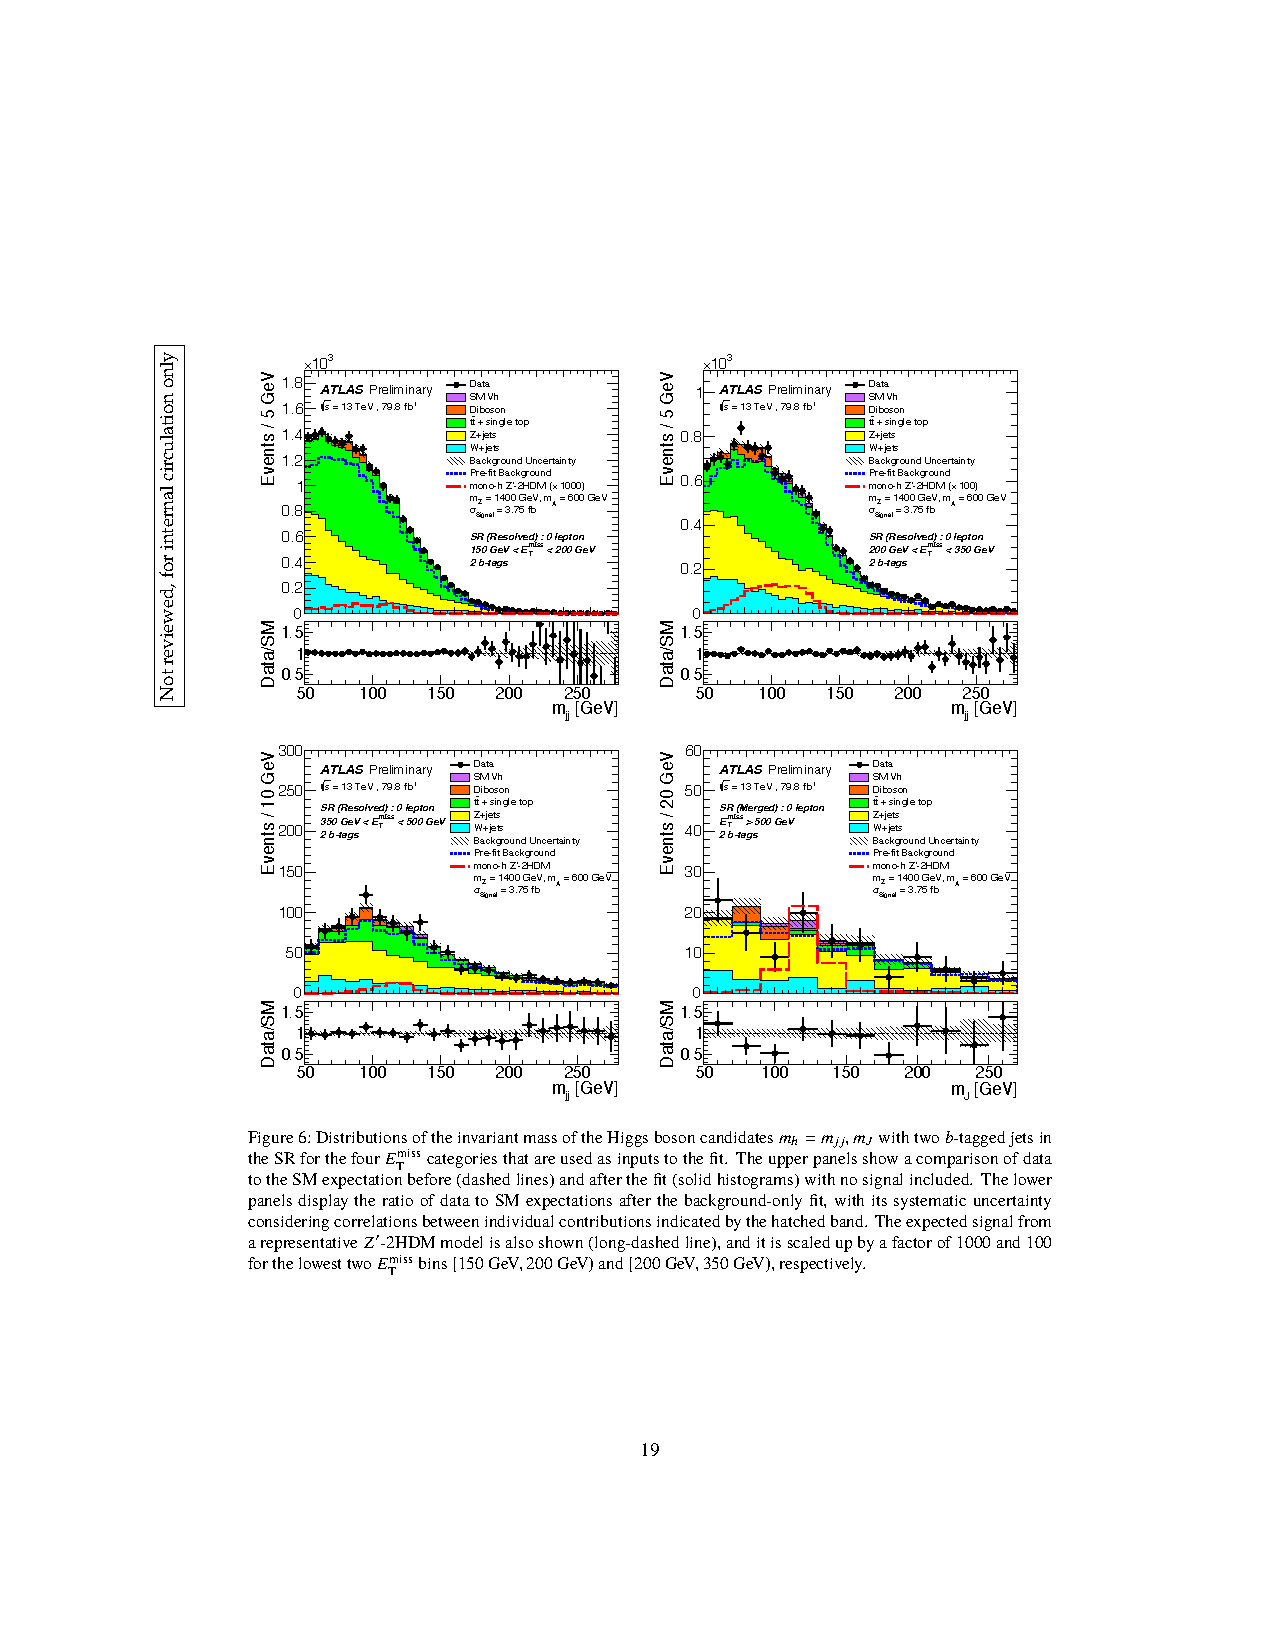
\includegraphics[width=13cm, trim={4cm 9cm 4cm 6cm}, clip]{chapters/c9/figures/post-fit-0lep.pdf}

  \caption{Distributions of the Higgs invariant mass with 2 b-tagged jets in the Signal Region with 79.8~\ifb data. The upper panels show a comparison of data to the SM expectation before (dashed lines) and after the fit (solid histograms) with no signal included. The lower
panels display the ratio of data to SM expectations after the background-only fit, with its systematic uncertainty considering correlations between 
    individual contributions indicated by the hatched band. The expected signal from a representative Z′-2HDM model is also shown (long-dashed line), 
    and it is scaled up by a factor of 1000 and 100 for the lowest two \met~bins [150 GeV, 200 GeV] and [200 GeV, 350 GeV], respectively.}
  \label{fig:Data_MC_SR_m_jj_2b_postfit}
  \end{figure}
  
\subsection{1-lepton (1L)}
\begin{figure}[H]
    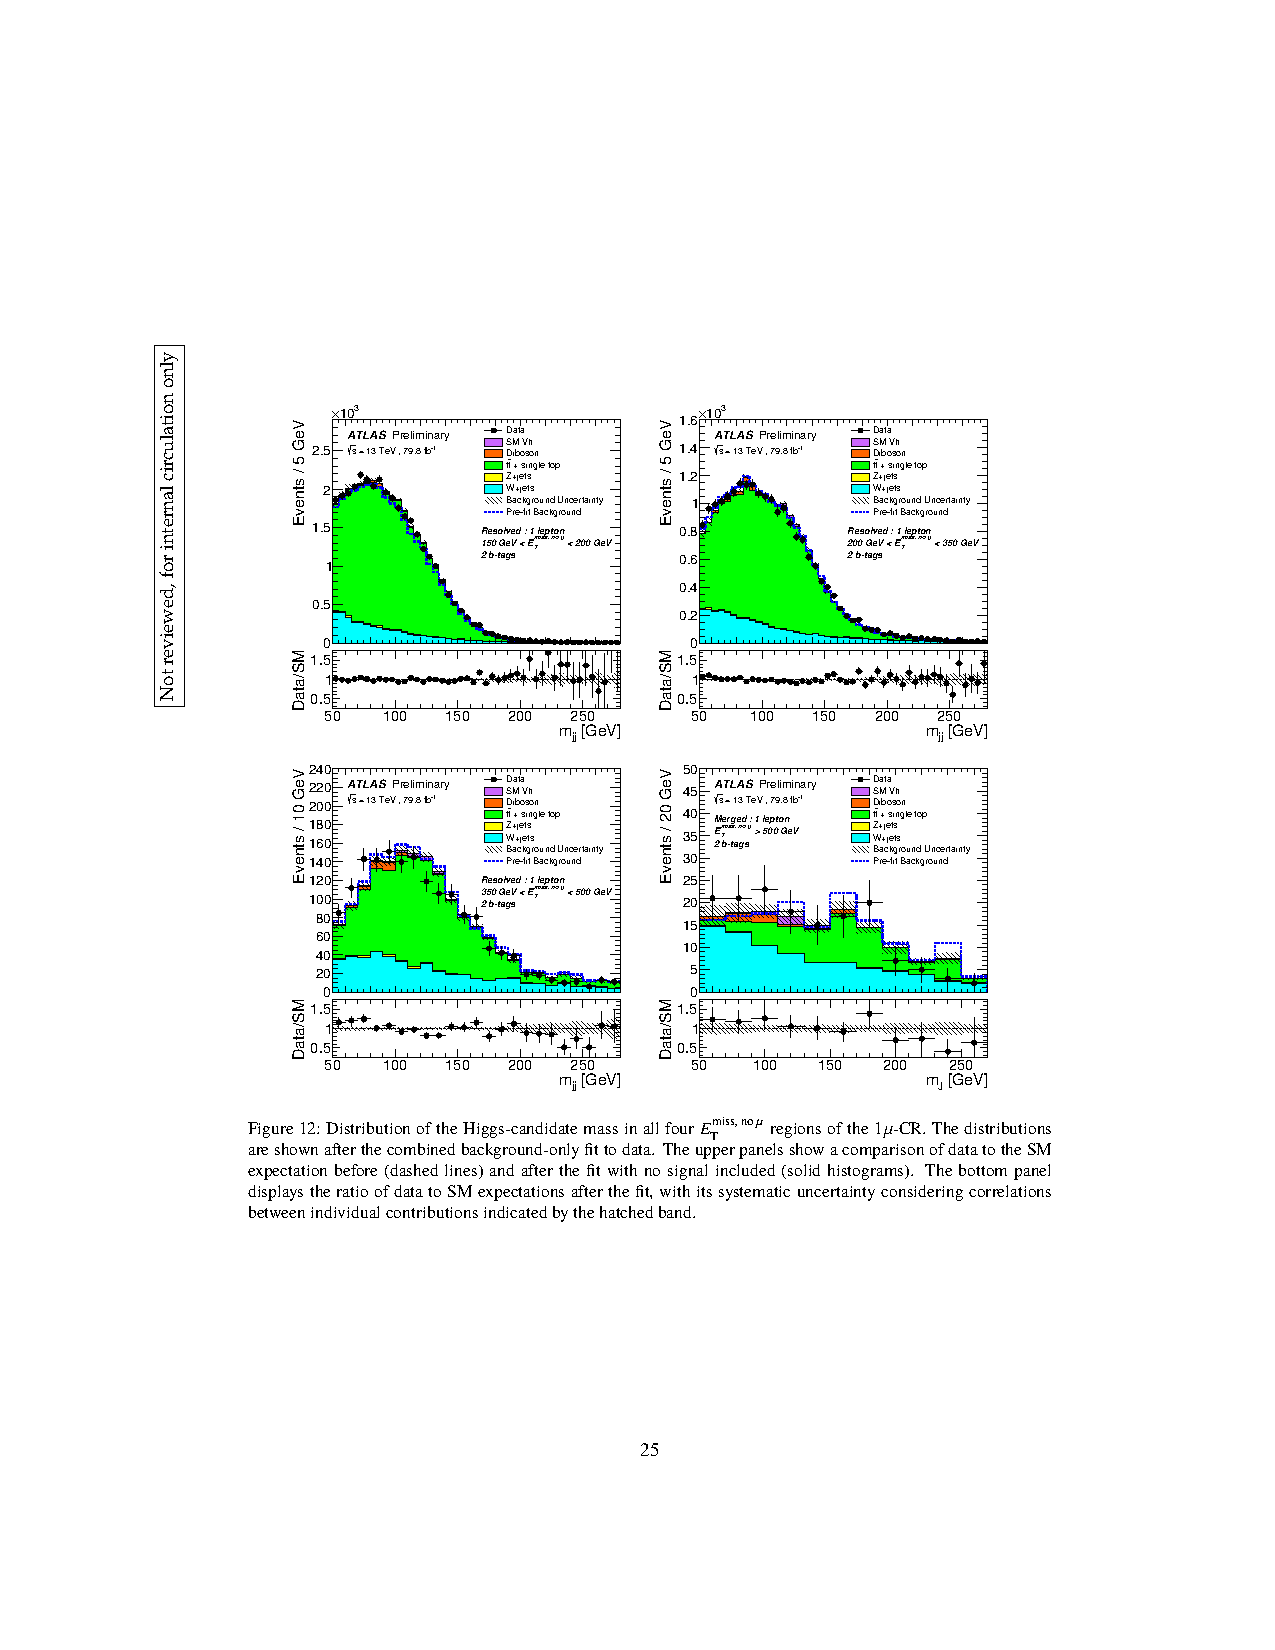
\includegraphics[width=15cm,trim={4cm 9cm 4cm 6cm}, clip]{chapters/c9/figures/post-fit-1lep.pdf}

  \caption{Distribution of the Higgs-candidate mass in 1 lepton Control Region with 79.8~\ifb data. The distributions are shown after the combined background-only fit to data. The upper panels show a comparison of data to the SM expectation before (dashed lines) and after the fit with no signal included (solid histograms). The bottom panel displays the ratio of data to SM expectations after the fit, with its systematic uncertainty considering correlations between individual contributions indicated by the hatched band.}
  \label{fig:Data_MC_CR1_mu_charge_2b_postfit}
\end{figure}

\subsection{2-lepton (2L)}
\begin{figure}[H]
    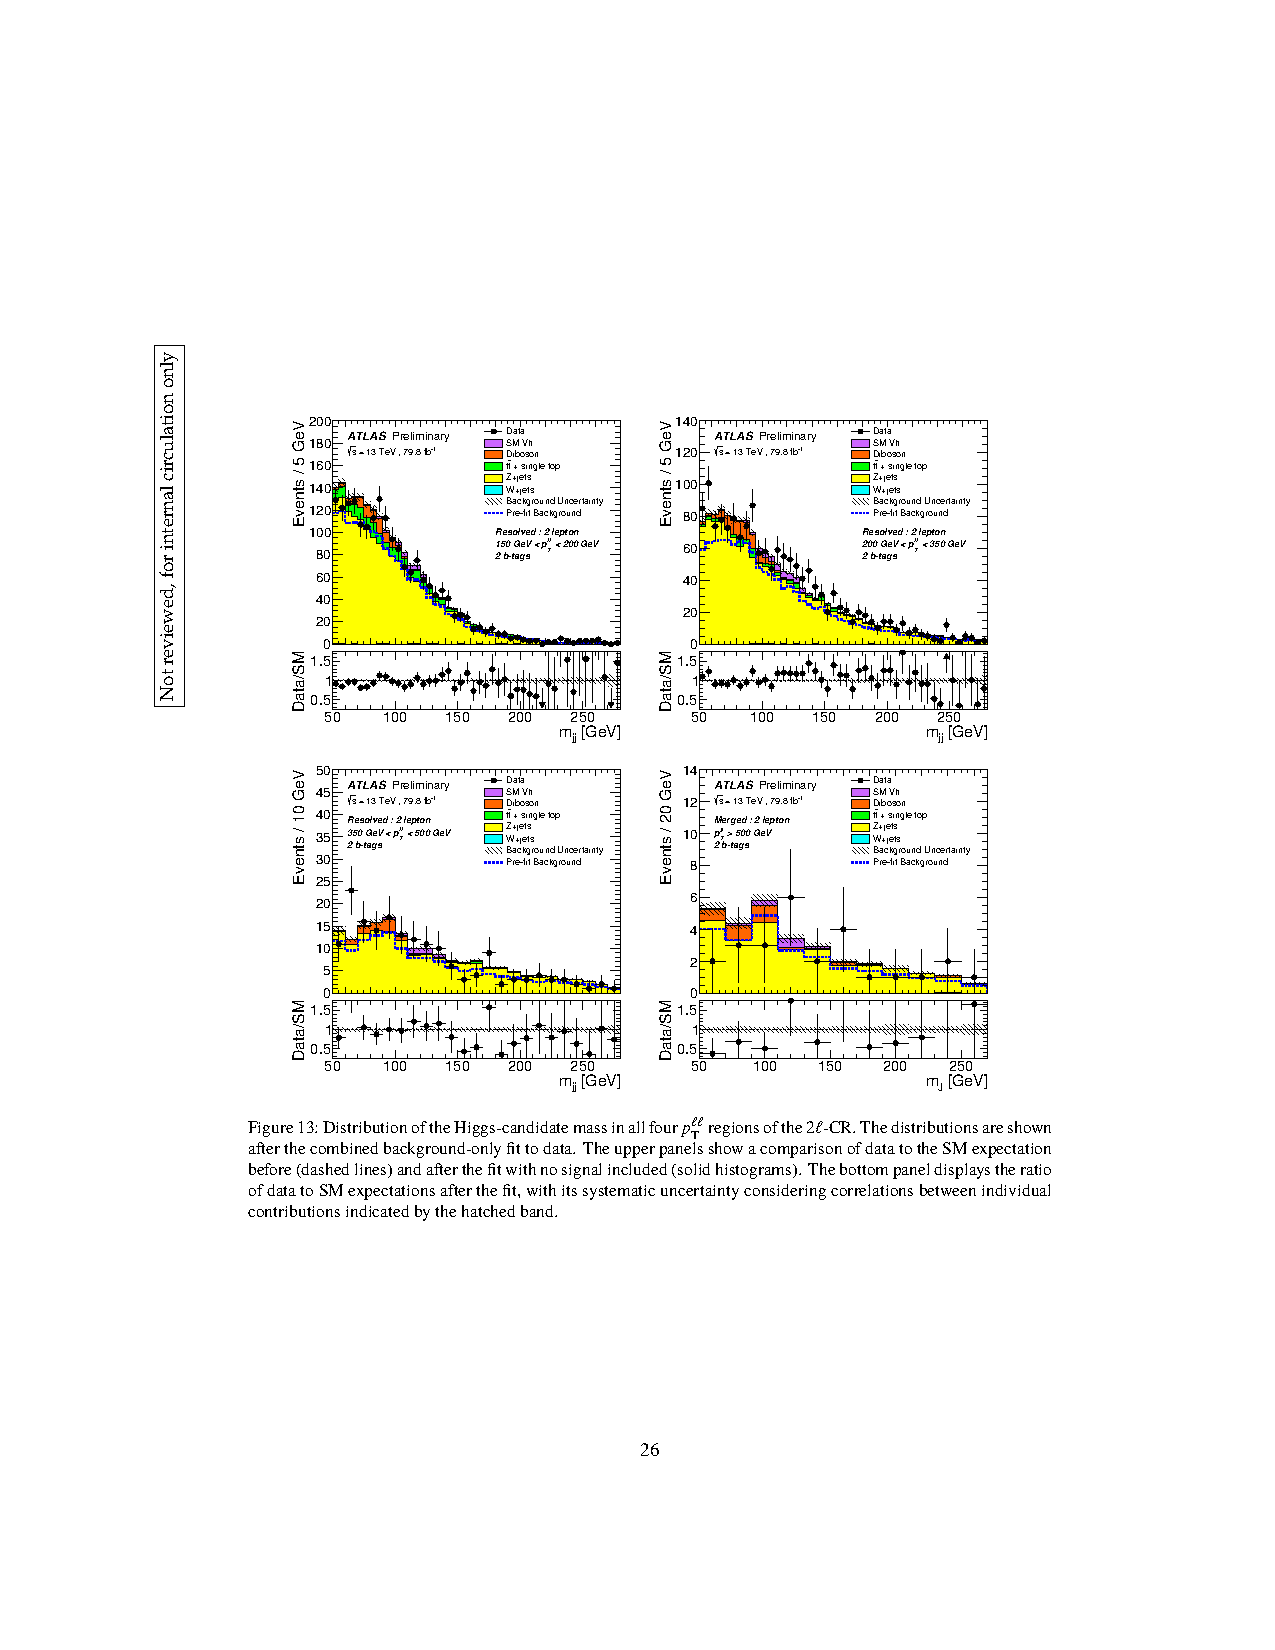
\includegraphics[width=15cm, trim={4cm 9cm 4cm 6cm}, clip]{chapters/c9/figures/post-fit-2lep.pdf}
  \caption{Distribution of the Higgs-candidate mass of the 2 lepton Control Region with 79.8~\ifb data. 
  The distributions are shown after the combined background-only fit to data. 
  The upper panels show a comparison of data to the SM expectation before (dashed lines) and after the fit with no signal included (solid histograms). 
  The bottom panel displays the ratio of data to SM expectations after the fit, with its systematic uncertainty considering correlations between individual contributions indicated by the hatched band.}
  
  
  \label{fig:Data_MC_CR2_ll_m_jj_2b_postfit}
\end{figure}


\section{Limit setting result}
\label{sec:limitres}

\par There are two interesting parameters in the Z'-2HDM: the mass of the Z' boson and the mass of the dark matter candidate A. 
Limit setting on the signal strength is implemented in a two dimensional scan on these two parameters.

\par The result is shown with 79.8~\ifb~unblinded data for the observed limits and expected limits in the Fig.~\ref{fig:zprime-2hdm-limit-80}. 
The result with 139~\ifb~scale are demonstrated in the Fig.~\ref{fig:zprime-2hdm-limit-139}. 
It indicates that the Z' mass epected to be excluded up to 2900~\GeV, 2700~\GeV~using data, while the A mass expected to be excluded up to 700~\GeV, while 650~\GeV~using data.

\begin{figure}[!htb]
    \centering
    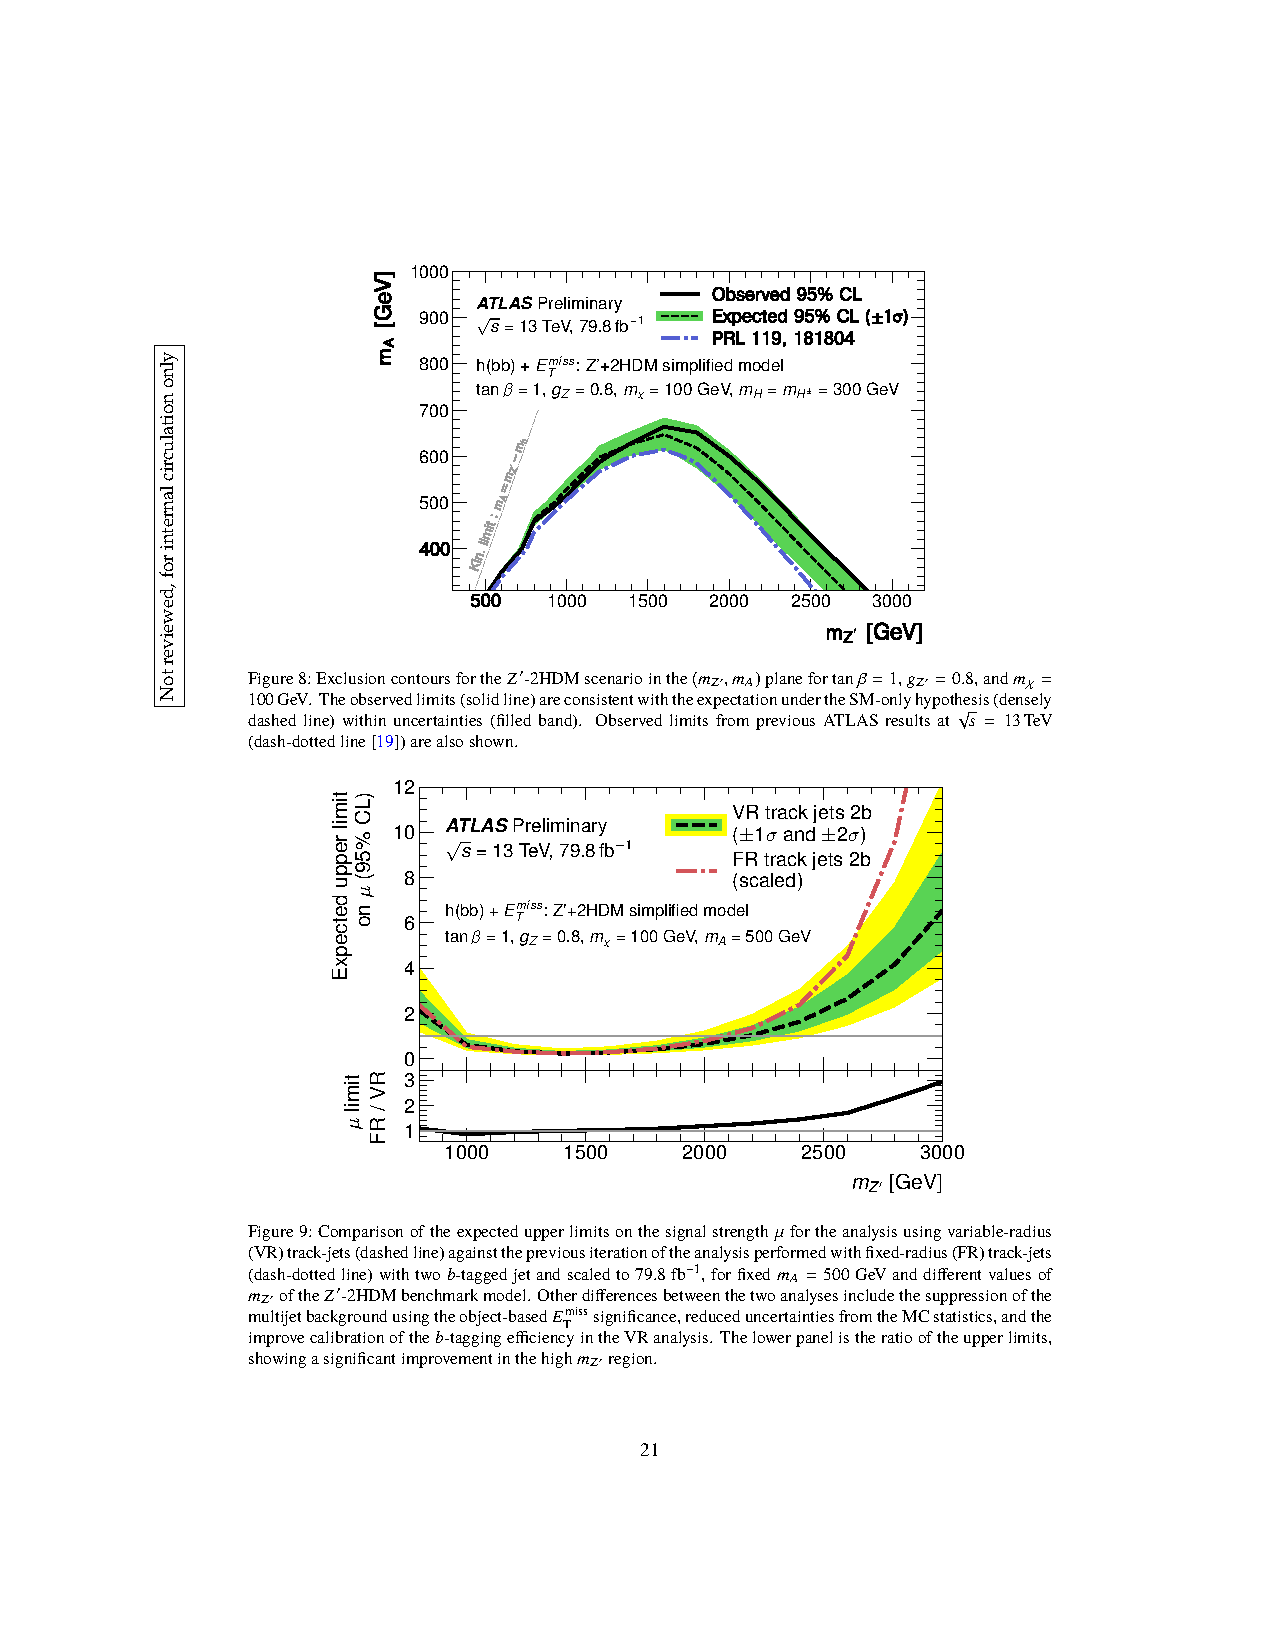
\includegraphics[width=12cm, height=9cm, trim={6cm 17cm 5.8cm 4.5cm}, clip]{chapters/c9/figures/ZPrime2HDMLimit-80Exp.pdf}
    \caption{Exclusion contours for the Z'-2HDM scenario in the ($m_{Z^{\prime}}$, $m_{A}$) plane for $tan\beta= 1$, $g_{Z^{\prime}}=0.8$, and $m_{\chi}=100$~\GeV. 
    The observed limits (solid line) are consistent with the expectation under the SM-only hypothesis (densely dashed line) within uncertainties (filled band). 
     Observed limits from previous ATLAS results at $\sqrt{s}=13~\TeV$ (dash-dotted line) are also shown. Both observed and expected limits are derived with 79.8~\ifb~data.}
    \label{fig:zprime-2hdm-limit-80}
\end{figure}



\begin{figure}[!htb]
    \centering
    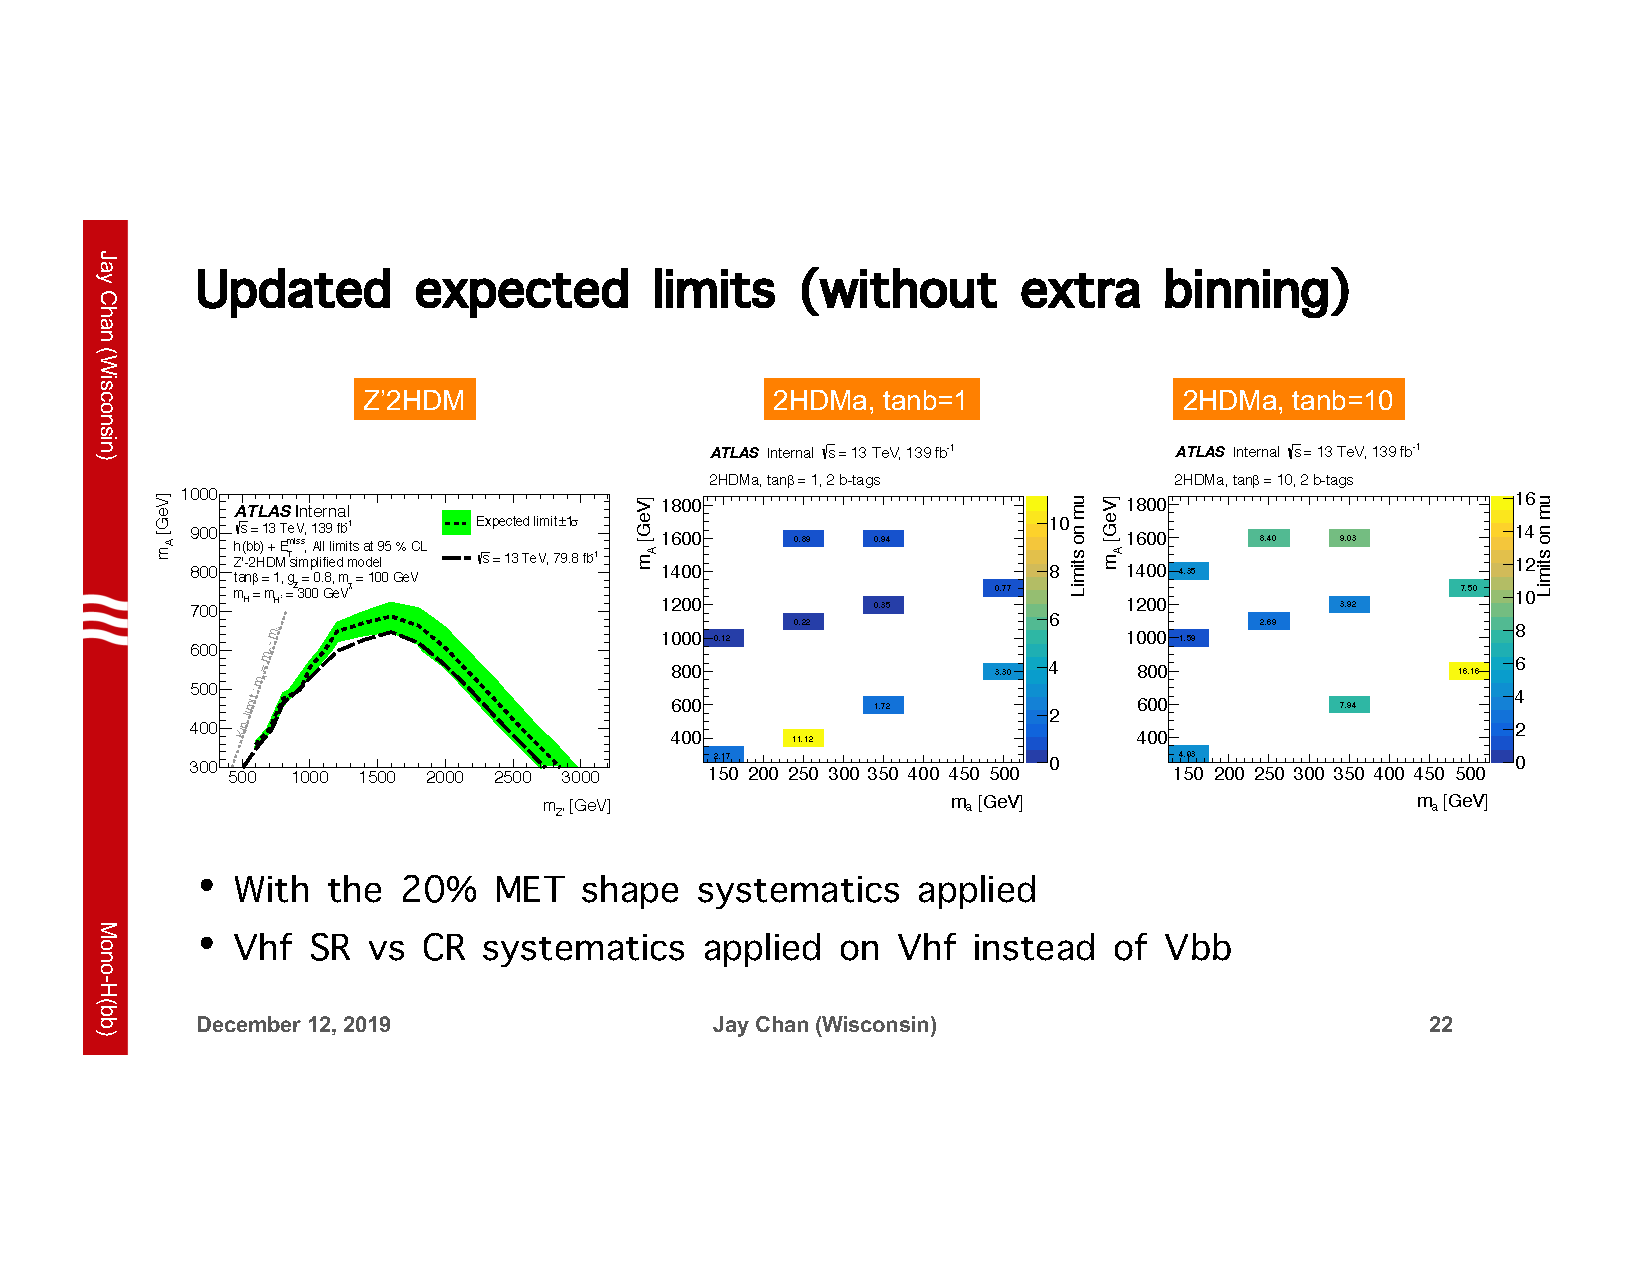
\includegraphics[width=12cm, height=9cm, trim={2.5cm 7.5cm 17.6cm 8cm}, clip]{chapters/c9/figures/ZPrime2HDMLimit-139Exp.pdf}
    \caption{Exclusion contours for the Z'-2HDM scenario in the ($m_{Z^{\prime}}$, $m_{A}$) plane for $tan\beta= 1$, $g_{Z^{\prime}}=0.8$, and $m_{\chi}=100$~\GeV. 
    The observed limits (solid line) are consistent with the expectation under the SM-only hypothesis (densely dashed line) within uncertainties (filled band). 
    The observed limits are derived with 79.8~\ifb~data, while the expected limits are with 139~\ifb~data.}
    \label{fig:zprime-2hdm-limit-139}
\end{figure}
